\documentclass[uplatex, dvipdfmx, a4paper, report, papersize, 11pt]{jsbook}
\usepackage{bm}
\usepackage{amsmath}
\usepackage[dvipdfmx]{graphicx}
\usepackage{wrapfig}
\usepackage[hang, small, bf]{caption}
\usepackage[subrefformat=parens]{subcaption}
\usepackage{here}
\usepackage{comment}
\captionsetup{compatibility=false}

\bibliographystyle{jplain}
\title{二色の光周波数コムによるレーザー冷却法の開拓}
\author{物理工学科4年 中西亮}
\date{2018/11/19}
\begin{document}
\maketitle
\newpage

\setcounter{tocdepth}{2}
\tableofcontents


\newpage
\chapter{序論}
\section{研究の背景と目的}
レーザー光の輻射圧を利用して原子の運動を抑制する技術であるレーザー冷却は原子物理において有用な手法として大きな役割を果たしている. 1980年以降, 研究が本格化したレーザー冷却は現在, ボースアインシュタイン凝縮の実現や光格子時計の精度向上, 量子情報処理への利用など様々な応用が研究されている. \cite{レーザー冷却とその応用}\par
しかし, 現在のレーザーで冷却することができる原子の種類は非常に限られており, 主にアルカリ金属, アルカリ土類金属の原子と希ガス原子の準安定状態である. \cite{PhysRevA.73.063407}この原因として, 多くの原子の冷却に必要とされる深紫外領域での高出力のcwレーザーを現状では実現できていないこと, 価電子の多い原子においては電子の遷移サイクルを実現するために多数のリポンプレーザーが必要となり光学系が複雑化してしまうことが挙げられる.\par
この問題を解決する手法の一つとして光周波数コムによる2光子遷移を利用したレーザー冷却の手法が提案されており, 実証実験も行われている\cite{PhysRevX.6.041004}\cite{PhysRevA.73.063407}. しかし、一種類のモード同期レーザーを用いた過去の実証実験の方法では、電子準位を近共鳴中間状態として用いることのできる原子は限られてしまう。そこでこの論文では、二色の光周波数コムを用いる構成に着目して、Cs原子を対象にその妥当性を検証し、実際に二色の光周波数コムを用いてレーザー冷却を実証することを目的とした。\\

\section{本論文の構成}

\newpage

\chapter{背景知識}

\section{ドップラー冷却}
\subsection{光が原子に及ぼす力}
 光が原子に及ぼす力は輻射圧と双極子力に分けることができる. 輻射圧は, 光子を吸収・放出する際に原子の運動量変化を起こす撃力である\cite{ノーベル賞と分光学}.
 電磁場の周波数を$\omega$, 原子の共鳴周波数を$\omega_0$としたとき, 波数$\bm k$の平面電磁場が速度$\bm v$の原子に与える平均輻射圧は,
 \begin{equation}\label{scattering_force}
\bm{F} _ { \mathrm { scatt } } = \hbar \bm{k}\frac { \Gamma } { 2 } \frac { \Omega ^ { 2 } / 2 } { \delta ^ { 2 } + \Omega ^ { 2 } / 2 + \Gamma ^ { 2 } / 4 }
 \end{equation}
となる\cite{Foot:1080846}. ただし, $\Gamma$は遷移の自然幅(半値全幅), $\Omega$は共鳴ラビ周波数, $\delta = \omega - \omega _ { 0 } - \bm{k} \cdot \bm{v}$はドップラー効果を考慮に入れた離調である. もう一つの力である双極子力は, 保存力であるために原子の捕獲はできるが冷却はできない\cite{ノーベル賞と分光学}.

\subsection{光糖蜜効果}
ドップラー冷却は原子の共鳴周波数に対して負の離調をつけた直交する3組の対向レーザーを, 原子に照射することで実現する. ある速度をもつ原子は, ドップラー効果により原子の運動と反対向きのレーザーの周波数をより高く感じ, 原子の運動と同じ向きのレーザーの周波数をより低く感じる. このため共鳴周波数に負の離調をつけた対向レーザーを原子に対して当てると, 原子は運動と反対むきのレーザーの輻射圧をより強く感じるので, 原子の速度は減速される. このように, 原子がレーザーを吸収するときに受ける力は常に運動の向きと逆向きであるが, 励起された原子が光子を自然放出する向きはランダムであるため自然放出による運動量の変化は平均すると無くなる. このため, 原子の運動は光子の吸収と放出を繰り返すことで抑えられていくことが分かる.\\
 輻射圧の式(\ref{scattering_force})から, 具体的に1組の対向ビームが原子に対して与える力を計算すると,
\begin{equation}
  \begin{split}
    F _ { \mathrm{molasses} } &= F _ { \mathrm{scatt}  } \left( \omega - \omega _ { 0 } - k v \right) - F _ {  \mathrm{scatt} }  \left( \omega - \omega _ { 0 } + k v \right)
    \\& \simeq F _ { \mathrm{scatt}  } \left( \omega - \omega _ { 0 } \right) - k v \frac { \partial F } { \partial \omega } - \left[ F _ {  \mathrm{scatt} } \left( \omega - \omega _ { 0 } \right) + k v \frac { \partial F } { \partial \omega } \right]
    \\& \simeq - 2 \frac { \partial F } { \partial \omega } k v
  \end{split}
\end{equation}
となる. この式を見ると, 対向ビームが原子に与える力は速度に比例する粘性抵抗の形をしていることが分かる.3組の対向ビームを当てると原子は粘性液体の中を動いているような振る舞いを見せる. このことからこの効果を初めて実証したChuらは, 「光糖蜜(Optical Molasses,  OM)効果」と呼んだ.

\subsection{ドップラー冷却限界}
 励起された原子は光子を自然放出する際に反跳を受ける.この反跳の向きが毎回ランダムなので原子はこの自然放出により加熱効果を受ける. また単位時間あたりに吸収する光子の数にも揺らぎがあるため, 原子にランダムな運動を引き起こす.
ドップラー冷却にはこのような加熱効果が存在し, 前述の冷却効果と均衡が取れるところがドップラー冷却で到達できる温度の限界となる. この温度$T _ { \mathrm { D } }$は
\begin{equation}
  k _ { \mathrm { B } } T _ { \mathrm { D } } = \frac { \hbar \Gamma } { 2 }
\end{equation}
で与えられる. ただし, $k _ { \mathrm { B } }$はボルツマン定数を表す.
\subsection{ドップラー冷却できる原子}
 ドップラー冷却は原理的にはどの原子に対しても使うことができるが, 実験上の制約から以下のような特徴をもつ原子に適用が制限される\cite{ノーベル賞と分光学}.
\begin{itemize}
  \item 光の吸収放出のサイクルが速い
  \item 冷却サイクルが閉じている.あるいは少数のレーザーで閉じることができる.
  \item 目的とする周波数帯に使いやすいレーザーが存在する.
\end{itemize}

\newpage


\section{磁気光学トラップ (MOT)}
 光糖蜜効果によるドップラー冷却では原子を減速させ冷却することはできるが, トラップすることはできない. 磁気光学トラップ(Magneto-Optical Trap,  MOT)は原子をトラップするための技術の一つである. MOTは図\ref{MOT_circular_polarization}のように, OMの3組の負の離調をつけた円偏光対向レーザーと, 一対のコイルに逆向きの電流を流すことで導入される四重極磁場(図\ref{MOT_magnetic_field})で構成される. 四重極磁場による原子準位のゼーマン分裂を利用して原子に加わる輻射圧に位置依存性をつけることで原子をトラップする.\\
 簡単な例として, 基底状態が$J = 0$, 励起状態が$J = 1$の遷移を考える.トラップの中心では磁場は$0$になり, 中心付近では磁場の大きさは中心からの変位に比例する. そのため, 四重極磁場によるゼーマン分裂は図\ref{MOT_zeeman_split}のようになる. また, 選択則により$\sigma^{+}(\sigma^{-})$の偏光は$m_J = 0$から$m_J = 1 (-1)$に励起する. 原子が$z > 0$の位置に移動すると, $m_J = -1$の準位のエネルギーが下がり、負の離調をつけた$\sigma^-$の輻射圧を強く受けてトラップの中心に押し戻される.$z < 0$に移動した時も同様の原理で中心に押し戻す力が働くことで原子がトラップされる.\\
  式(\ref{scattering_force})を用いて, 原子に及ぼされる輻射圧を計算すると,
\begin{equation}
  \begin{aligned}
     F _ { \mathrm { MOT } } & = F _ { \mathrm { scatt } } ^ { \sigma ^ { + } } \left( \omega - k v - \left( \omega _ { 0 } + \beta z \right) \right) - F _ { \mathrm { scatt } } ^ { \sigma ^ { - } } \left( \omega + k v - \left( \omega _ { 0 } - \beta z \right) \right) \\ & \simeq - 2 \frac { \partial F } { \partial \omega } k v + 2 \frac { \partial F } { \partial \omega _ { 0 } } \beta z
  \end{aligned}
\end{equation}
となる. ここで$\beta z$の項はゼーマンシフトを表し,
\begin{equation}
  \beta z = \frac { g \mu _ { \mathrm { B } } } { \hbar } \frac { \mathrm { d } B } { \mathrm { d } z } z
\end{equation}
ただし, ここでは$g = g _ { J }$でランデの$g$因子を表し, $\mu _ { \mathrm { B }}$はボーア磁子である. いま, 力は$\delta = \omega - \omega _ { 0 }$に依存しているので, $\partial F / \partial \omega _ { 0 } = - \partial F / \partial \omega$より,
\begin{equation}
  \begin{aligned} F _ { \mathrm { MOT } } & = - 2 \frac { \partial F } { \partial \omega } ( k v + \beta z ) \\ & = - \alpha v - \frac { \alpha \beta } { k } z \end{aligned}
\end{equation}
となる. ただし$\alpha = 2\frac{\partial F}{\partial \omega} k$である. この表式から, MOT中の原子には復元力と粘性抵抗の形で表される力が働いていることが分かる.
\newpage

\begin{comment}
\begin{figure}[htbp]
 \begin{center}
  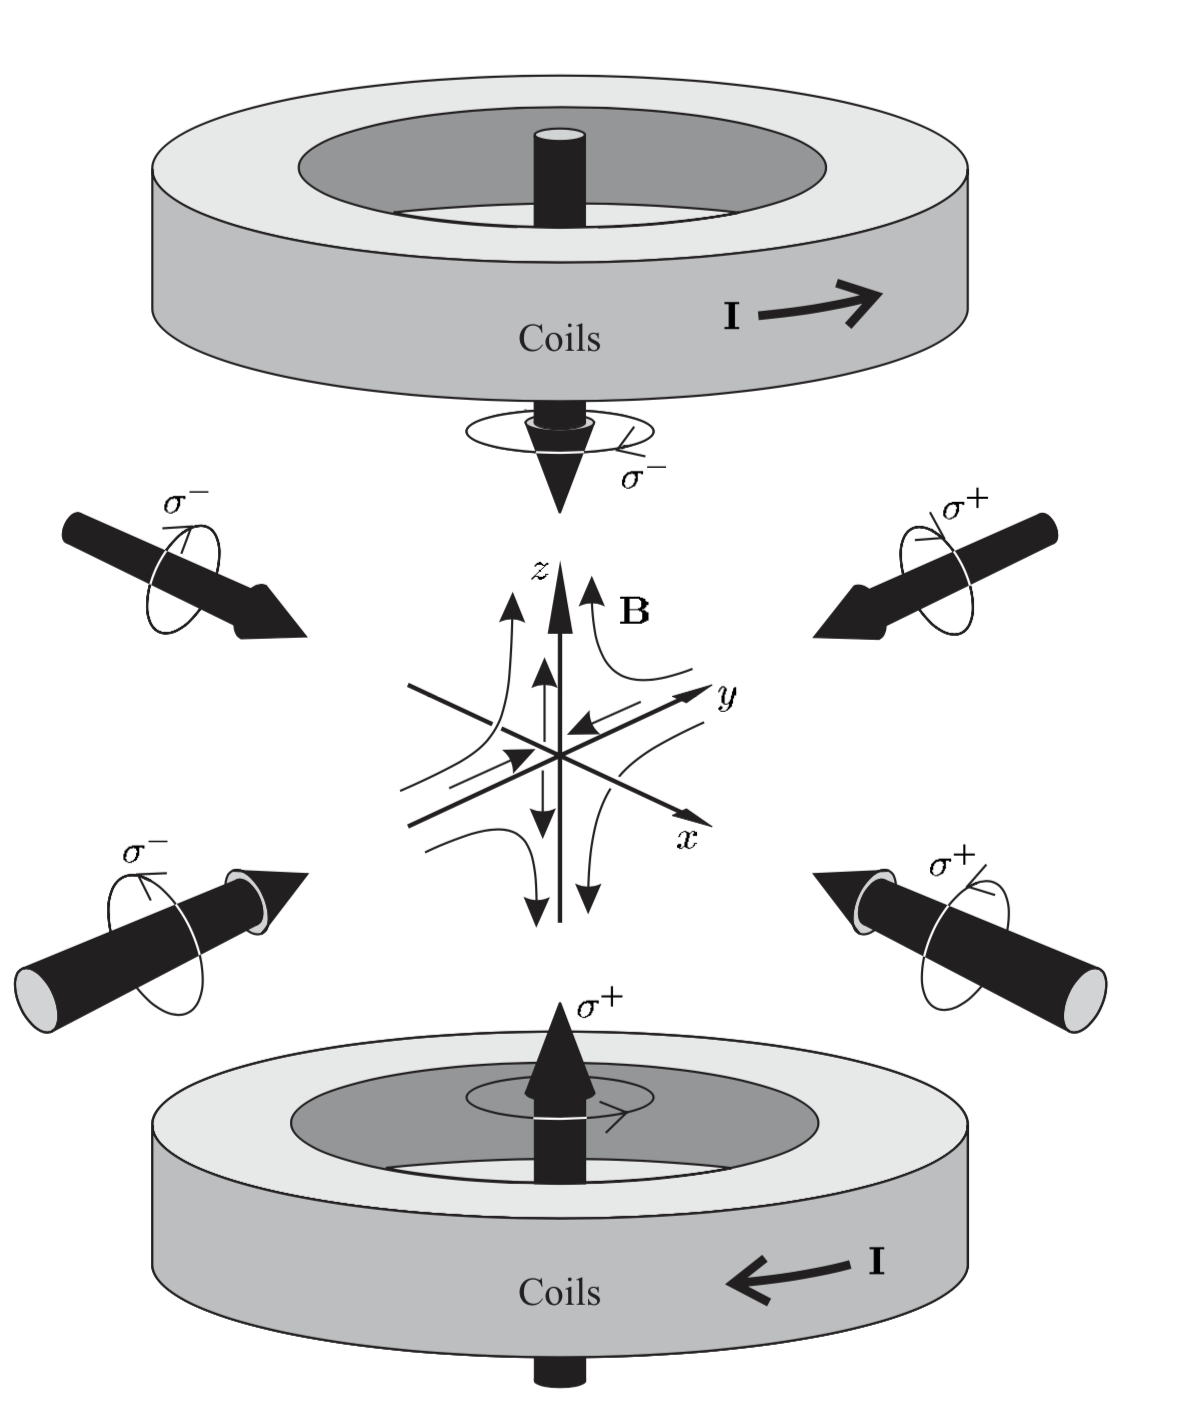
\includegraphics[width=40mm]{figures/MOT_circular_polarization.png}
\end{center}
 \caption{MOT}
 \label{MOT_circular_polarization}
\end{figure}

\begin{figure}[htbp]
 \begin{center}
  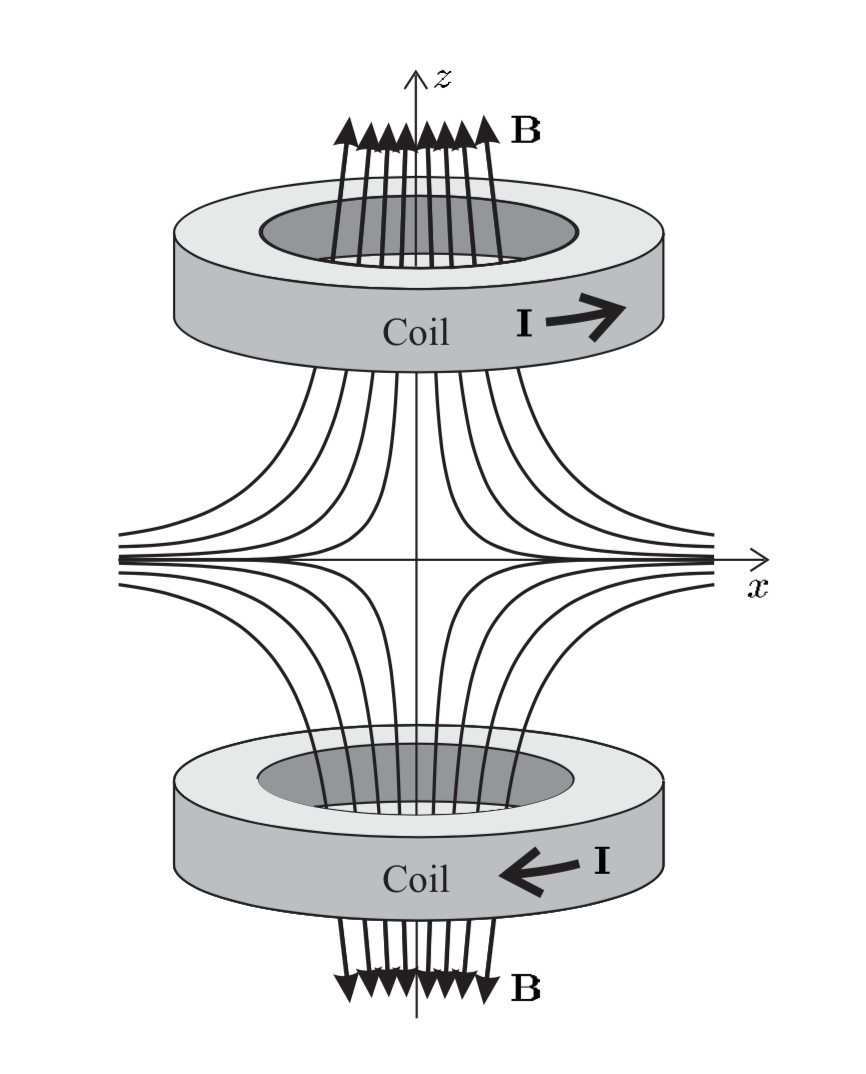
\includegraphics[width=50mm]{figures/MOT_magnetic_field.png}
\end{center}
 \caption{四重極磁場}
 \label{MOT_magnetic_field}
\end{figure}

\begin{figure}[htbp]
 \begin{center}
  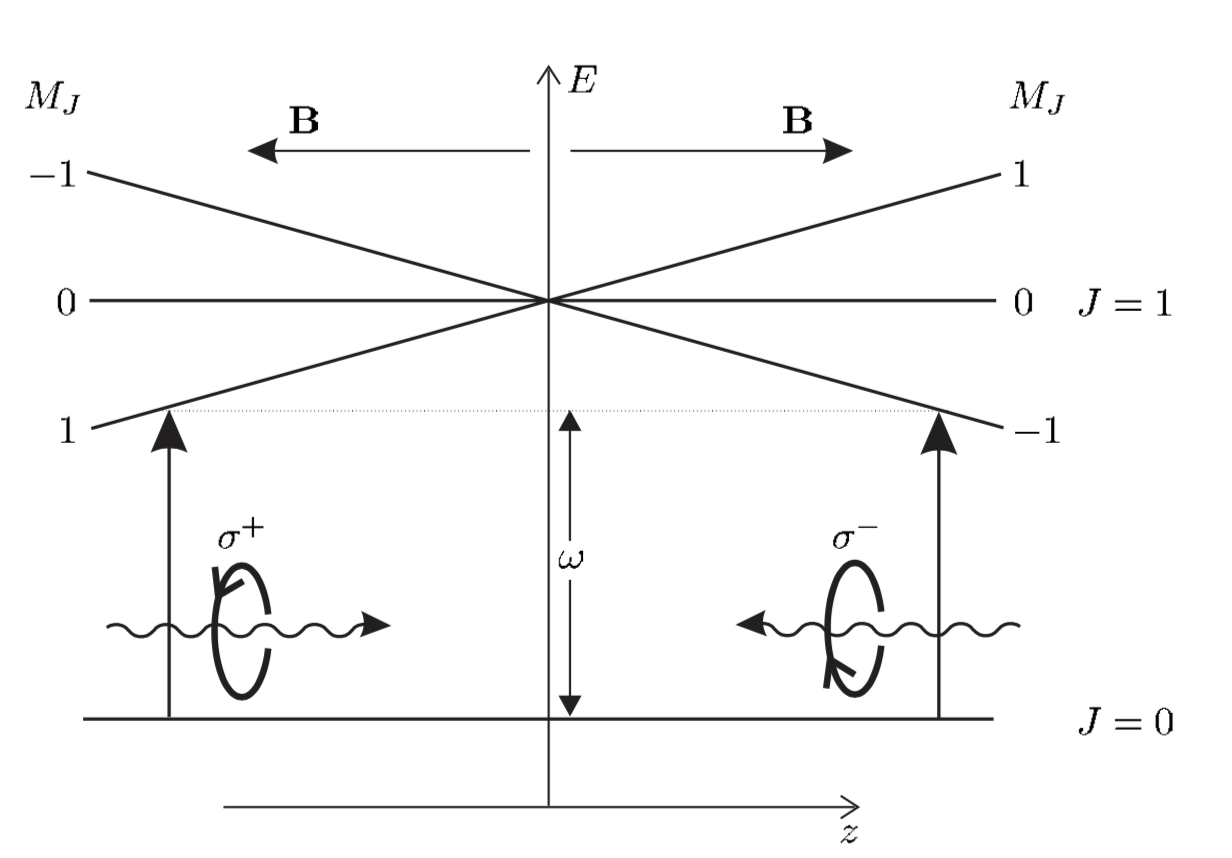
\includegraphics[width=50mm]{figures/MOT_zeeman_split.png}
 \end{center}
 \caption{四重極磁場によるゼーマン分裂}
 \label{MOT_zeeman_split}
\end{figure}
\end{comment}


\begin{figure}[htpb]
  \centering
    \begin{tabular}{c}

%----- MOTの構成 -----

      \begin{minipage}{0.50\hsize}
        \centering
          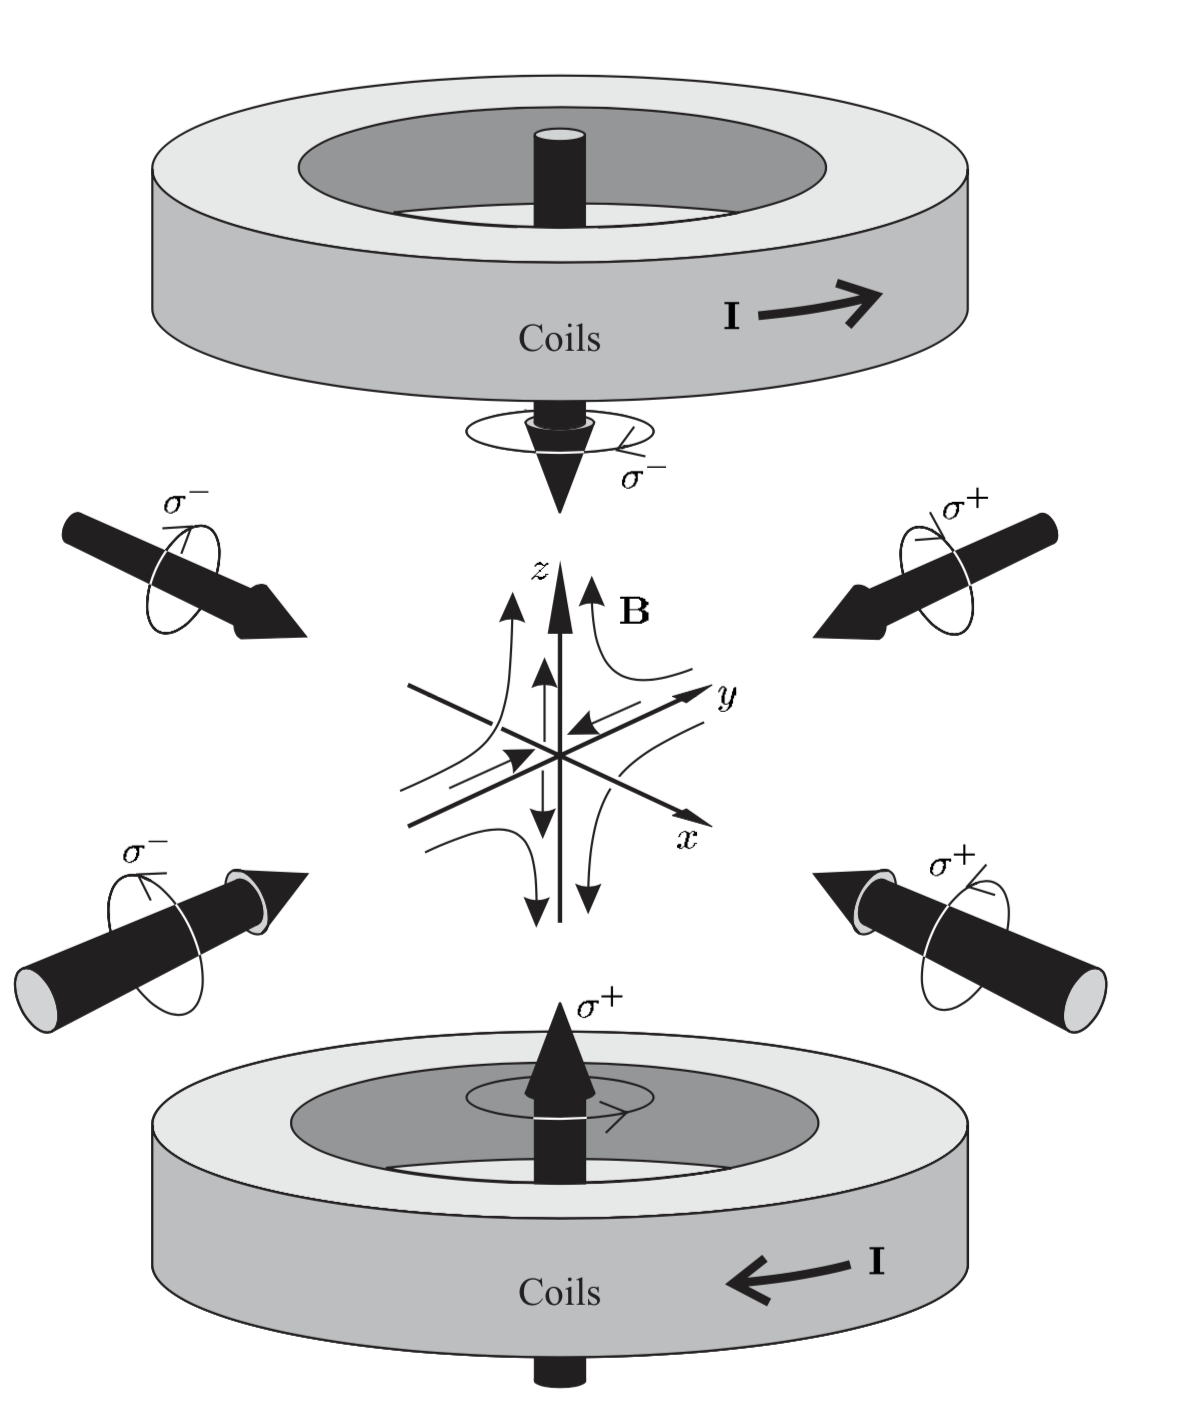
\includegraphics[keepaspectratio,  scale=0.35,  angle=0]
                          {figures/chapter2/MOT_circular_polarization.png}
                          \caption{MOTの構成(文献\cite{Foot:1080846}より引用)}
                          \label{MOT_circular_polarization}
      \end{minipage}

%----- 四重極磁場 -----

      \begin{minipage}{0.50\hsize}
        \centering
          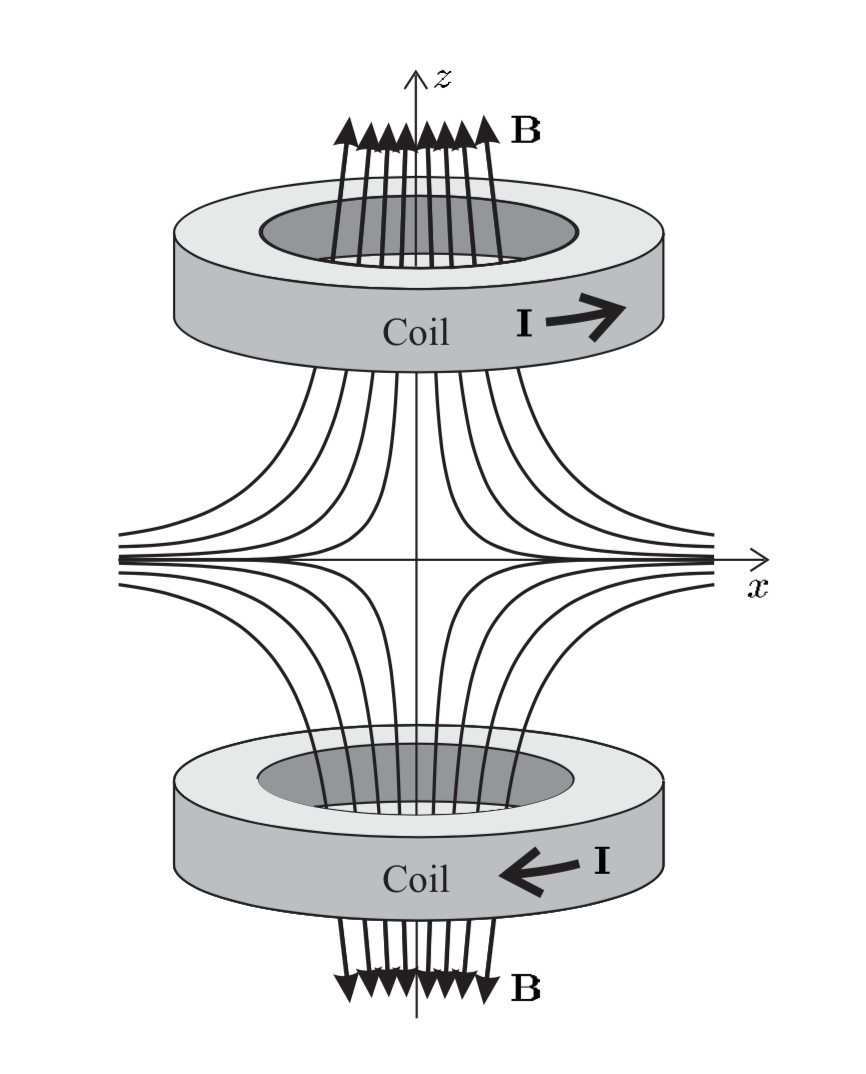
\includegraphics[keepaspectratio,  scale=0.50,  angle=0]
                          {figures/chapter2/MOT_magnetic_field.png}
                          \caption{四重極磁場(文献\cite{Foot:1080846}より引用)}
                          \label{MOT_magnetic_field}
      \end{minipage} \\

%-----四重極磁場によるゼーマン分裂 -----

      \begin{minipage}{0.50\hsize}
        \centering
          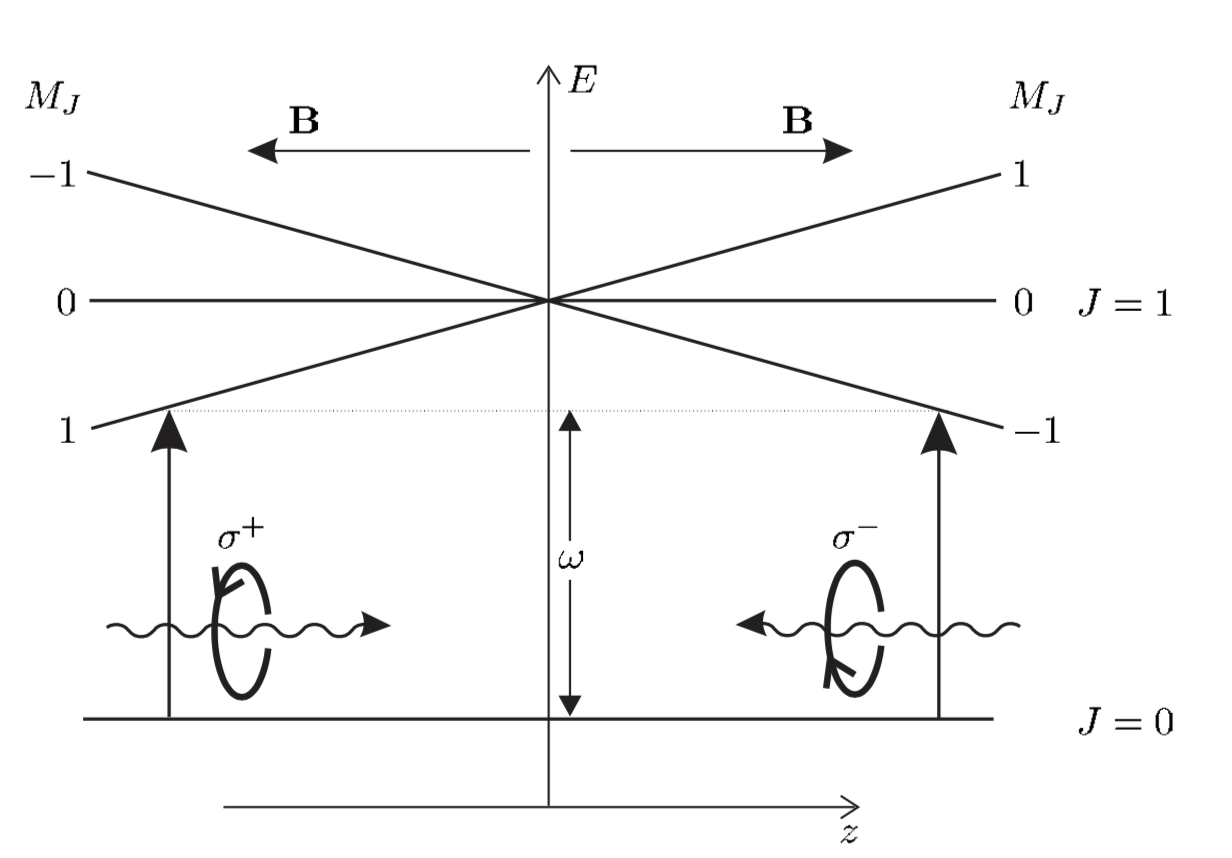
\includegraphics[keepaspectratio,  scale=0.40,  angle=0]
                          {figures/chapter2/MOT_zeeman_split.png}
                          \caption{四重極磁場によるゼーマン分裂(文献\cite{Foot:1080846}より引用)}
                          \label{MOT_zeeman_split}
      \end{minipage}


    \end{tabular}
\end{figure}

\newpage
\section{飽和吸収分光法}
\subsection{原理}
今回の実験の目標はコムでレーザー冷却をすることで、まずcw光によるMOTを構成しそこにコムの光を当てる。ここで、MOTを構成するために使うcw光の周波数をロックするために「飽和吸収分光法」を利用している. 通常の分光法では原子の遷移周波数の線幅は, 温度に応じたドップラー拡がりを持っている. これに対し, 飽和吸収分光法はドップラー拡がりを克服し, 原子の遷移周波数を測定する手法である. \\図\ref{saturated_absorption_figure}のように, レーザーをポンプ光とプローブ光に分けて原子の気体が入ったセルに照射し, プローブ光のセルの透過強度を測定する.\\
レーザーの周波数が原子の共鳴周波数$\omega_0$に合っているとき, レーザーの進行方向に対して速度ゼロ近傍の原子が平均パワーの大きなポンプ光によって吸収飽和を生じているため, セル通過後のプローブ光はポンプ光の影響を受けてあまり原子に吸収されない。レーザーの周波数が$\omega_0$からずれているときは、吸収飽和を生じているのは有限のドップラーシフトをもつ原子であるため、逆方向から進行してくるプローブ光に対してはポンプ光の影響はない。この効果により、レーザーの周波数を掃引すると、プローブ光の透過光強度は図図\ref{PD_Signal_main}のようになり、ドップラーフリーの吸収スペクトルを得ることができる。
\subsection{クロスオーバー共鳴}
 飽和吸収分光においては、準位間の共鳴周波数だけでなく二つの共鳴周波数のちょうど平均の周波数においてもプローブ光の透過率が極大となる。この現象をクロスオーバー共鳴と呼ぶ。もっとも簡単な三準位の系での飽和吸収分光を考える。図の$|1\rangle$から$|2\rangle$,$|3\rangle$への遷移周波数を$\omega_12$, $\omega_13$とする。レーザーの周波数が$\omega$のときに$|1\rangle$から$|2\rangle$へ励起される原子の速度は$v = \pm frac{\omega - \omega_12}{k}$であり、同様に$v = \pm frac{\omega - \omega_13}{k}$の速度の原子が$|3\rangle$へ励起される。
$\omega = \frac{\omega_12 + \omega_13}{2}$のとき、$|2\rangle$、$|3\rangle$へ励起される原子の速度が一致する。このため、$\omega_12$、$\omega_13$においてだけでなく、$\frac{\omega_12 + \omega_13}{2}$においてもポンプ光による飽和の影響でプローブ光の透過率が極大となることが分かる。
\begin{figure}[htpb]
  \centering
    \begin{tabular}{c}

%----- 写真 -----

      \begin{minipage}{0.50\hsize}
        \centering
          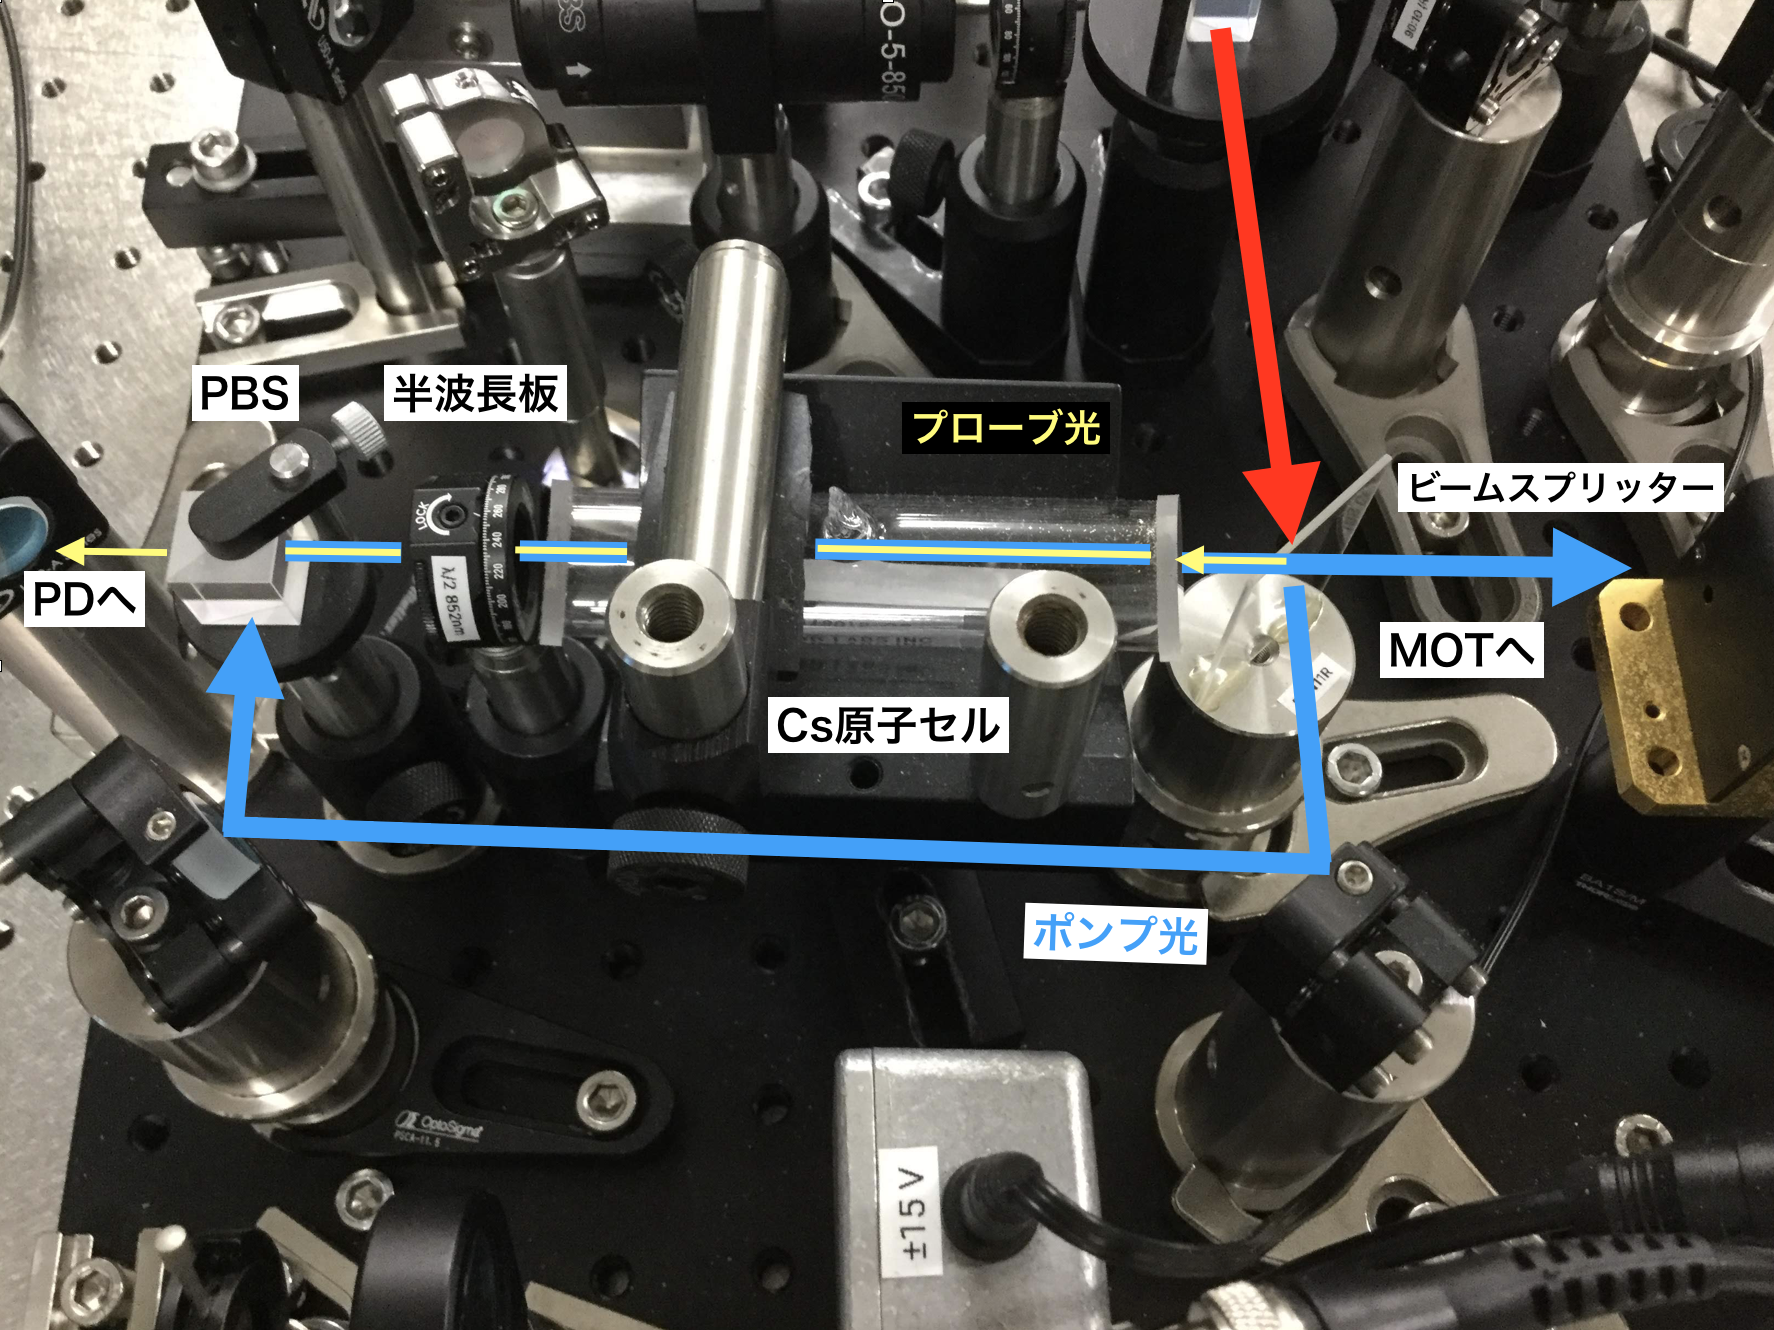
\includegraphics[keepaspectratio,  scale=0.20,  angle=0]
                          {figures/chapter2/saturated_absorption_figure.png}
                          \caption{飽和吸収分光の光学系\\
                          ただし、PBSはPolarization Beam Splitter、PDはPhoto Detectorを意味する。}
                          \label{saturated_absorption_figure}
      \end{minipage}

%----- PD Signal -----

      \begin{minipage}{0.50\hsize}
        \centering
          \includegraphics[keepaspectratio,  scale=0.5,  angle=0]
                          {figures/chapter2/PD_Signal_main.png}
                          \caption{飽和吸収分光によって観測されたCsの超微細構造}
                          \label{PD_Signal_main}
      \end{minipage} \\

    \end{tabular}
\end{figure}



\section{光周波数コム}
\subsection{モード同期レーザーの概要}
今回の実験で光源として用いられているモード同期レーザーは, 時間的に等間隔で出力されるパルス列である. このパルス列は共振器内の異なる縦モードの位相を同期することで得られる. モード同期の手法には能動的モード同期と受動的モード同期があるが, 今回の実験では受動的モード同期を用いている.\\
 受動的モード同期法は共振器内に可飽和吸収体を設置することで行われる. これは強度が弱い光は吸収するが, 高強度の光に対しては飽和を起こし高い透過率を示すような素子である. これによりパルスの裾では吸収が起こりパルスの頂点付近では吸収が起きないため, パルスの持続時間を短く保つことができる. このようにして, モード同期が自発的に行われる.\\
 レーザーの利得媒質としてチタンサファイア(Ti:Sa)を用いると, Ti:Sa自体が可飽和吸収体として振る舞う.これはTi:Sa中で起こるカーレンズ効果により, パルスの頂点付近の高強度の光は細くなりスリットを損失なく通過するが裾野の光はスリットで損失を受けるためTi:Saが実効的な可飽和吸収体として振る舞うためである.\\
 また, 共振器内のミラーや利得媒質による群速度分散をプリズムやミラーで補償することで短パルスを維持する手法も用いられている. このように、フェムト秒パルス光の方がレーザー共振器内の損失が小さくなる効果と、分散媒質をフェムト秒パルス光が通過する際に不可避であるチャープなどの分散の影響を補償することによって、フェムト秒パルス光が安定に発振するレーザーを実現できる。
\subsection{モード同期レーザーのスペクトル}
 モード同期レーザーの周波数領域でのスペクトルは等間隔のピークを持つ櫛状の形状となり, その周波数は
\begin{equation}
  f = nf_{\mathrm{rep}} + f_{\mathrm{ceo}}
\end{equation}
と表される\cite{Femtosecondopticalfrequencycombs}. $n$は整数である。ここで$f_{\mathrm{rep}}$は繰り返し周波数, $f_{\mathrm{ceo}}$はキャリア・エンベロープ・オフセット周波数と呼ばれる.このようなスペクトルの形状からモード同期レーザーは光周波数コムとも呼ばれる.\\
 また, $f_{\mathrm{ceo}}$はパルス間の位相のシフトに対応しており,
 \begin{equation}
   f _ { 0 } = \frac { 1 } { 2 \pi } f _ { \mathrm { rep } } \Delta \phi _ { \mathrm { ce } }
 \end{equation}
と表される\cite{Femtosecondopticalfrequencycombs}. ここで, $\Delta \phi _ { \mathrm { ce } }$はパルス間でのキャリアと包絡関数の位相差の変化を表す. $\Delta \phi _ { \mathrm { ce } }$は, 共振器内の分散による群速度と位相速度の差から生まれる. パルスは共振器内を一周する度に出力されるため, 位相の変化は
\begin{equation}
  \Delta \phi _ { \mathrm { ce } } = \left( \frac { 1 } { \nu _ \mathrm{ g } } - \frac { 1 } { \nu _ \mathrm{ p } } \right) l _ \mathrm{ c } \omega _ \mathrm{ c }\ (\bmod 2 \pi)
\end{equation}
と表される\cite{Femtosecondopticalfrequencycombs}. ただし, $\nu _ \mathrm{ g }$, $\nu _ \mathrm{ p }$はそれぞれ群速度, 位相速度を表し, $l_c$は共振器長, $\omega_c$はキャリア周波数を表す.
\section{テーパーアンプ}
今回の実験では光周波数コムの光をテーパーアンプ(Tapered Amplifier,  TA)で増幅しているが, この節ではTAの原理について説明する.

\subsection{半導体レーザーの発光原理}
TAは半導体で構成されており, その発光原理は半導体レーザーと同様であり構造も非常に似通っている. このため, まず文献\cite{わかる半導体レーザーの基礎と応用}の議論に沿って, 半導体レーザーの発光原理について説明する. 半導体レーザーの基本構造は図\ref{semicon_structure}のように, 3層のサンドイッチ構造で出来ており, 真ん中に挟まれ発光する層を「活性層」, 活性層を挟み込んで光やキャリアを閉じ込める役割を担う二つの層を「クラッド層」と呼ぶ. このような構造をDH(Double Hetero)構造と呼ぶ.\\
 この半導体p-n接合のエネルギーバンド構造は図\ref{semicon_bands}のようになる. 半導体レーザーでは図\ref{semicon_bands}のように電子が伝導帯から価電子帯に落ちる際のエネルギー差に相当する光が放出されるが, バンド間遷移であるためにライン間遷移に比べ発光スペクトルは広い. この素子に図\ref{semicon_structure}のように順方向のバイアスをかけるとエネルギーバンドが平らになっていき, p-n接合領域に電子とホールが集まり反転分布が形成される. このバンドギャップはGaAsの場合, 約$1.4$ eVで$800$ nmから$900$ nmに相当する\cite{grynberg_aspect_fabre_cohen-tannoudji_2010}. 半導体レーザーでは活性層の両へき界面に鏡をコーティングすることで光フィードバックを実現しレーザー動作を可能としている.

\begin{figure}[htpb]
  \centering
    \begin{tabular}{c}

%----- 半導体レーザーの構造 -----

      \begin{minipage}{0.70\hsize}
        \centering
          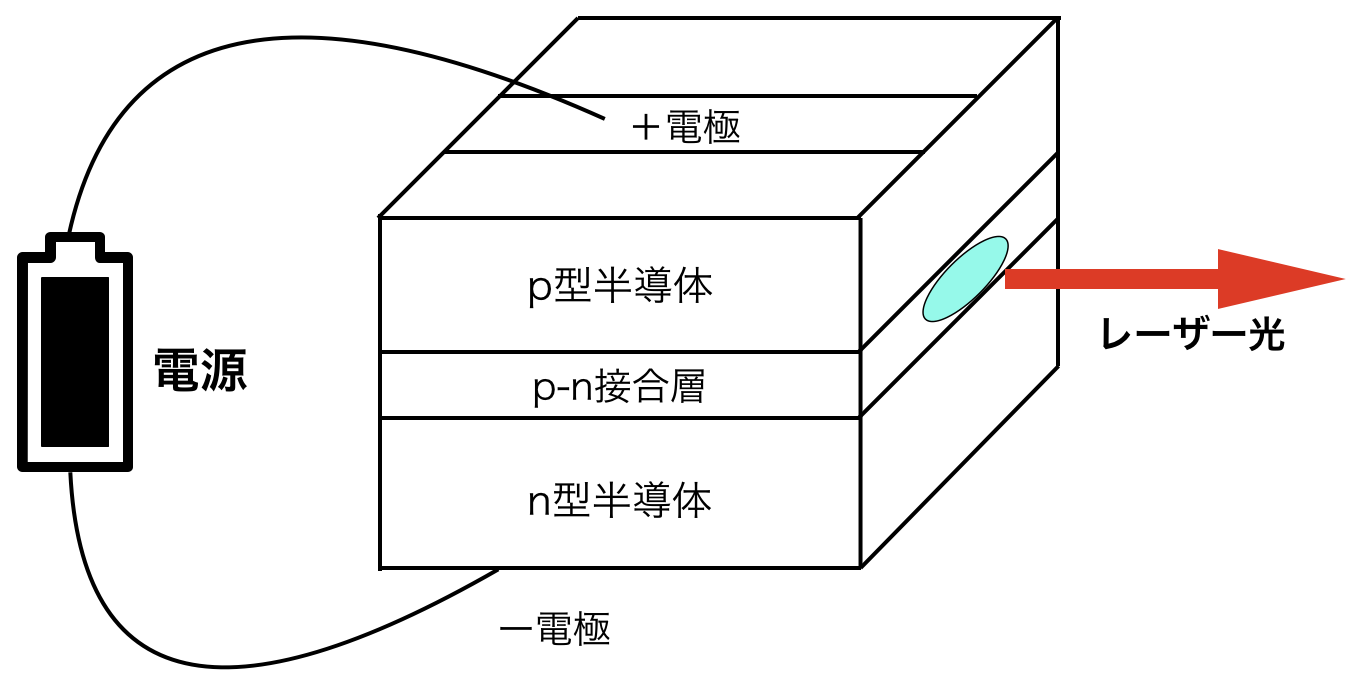
\includegraphics[keepaspectratio,  scale=0.35,  angle=0]
                          {figures/chapter2/semicon_structure.png}
                          \caption{半導体レーザーの基本構造}
                          \label{semicon_structure}
      \end{minipage}\\
      \\
      \\

%----- バンド図 -----

      \begin{minipage}{0.70\hsize}
        \centering
          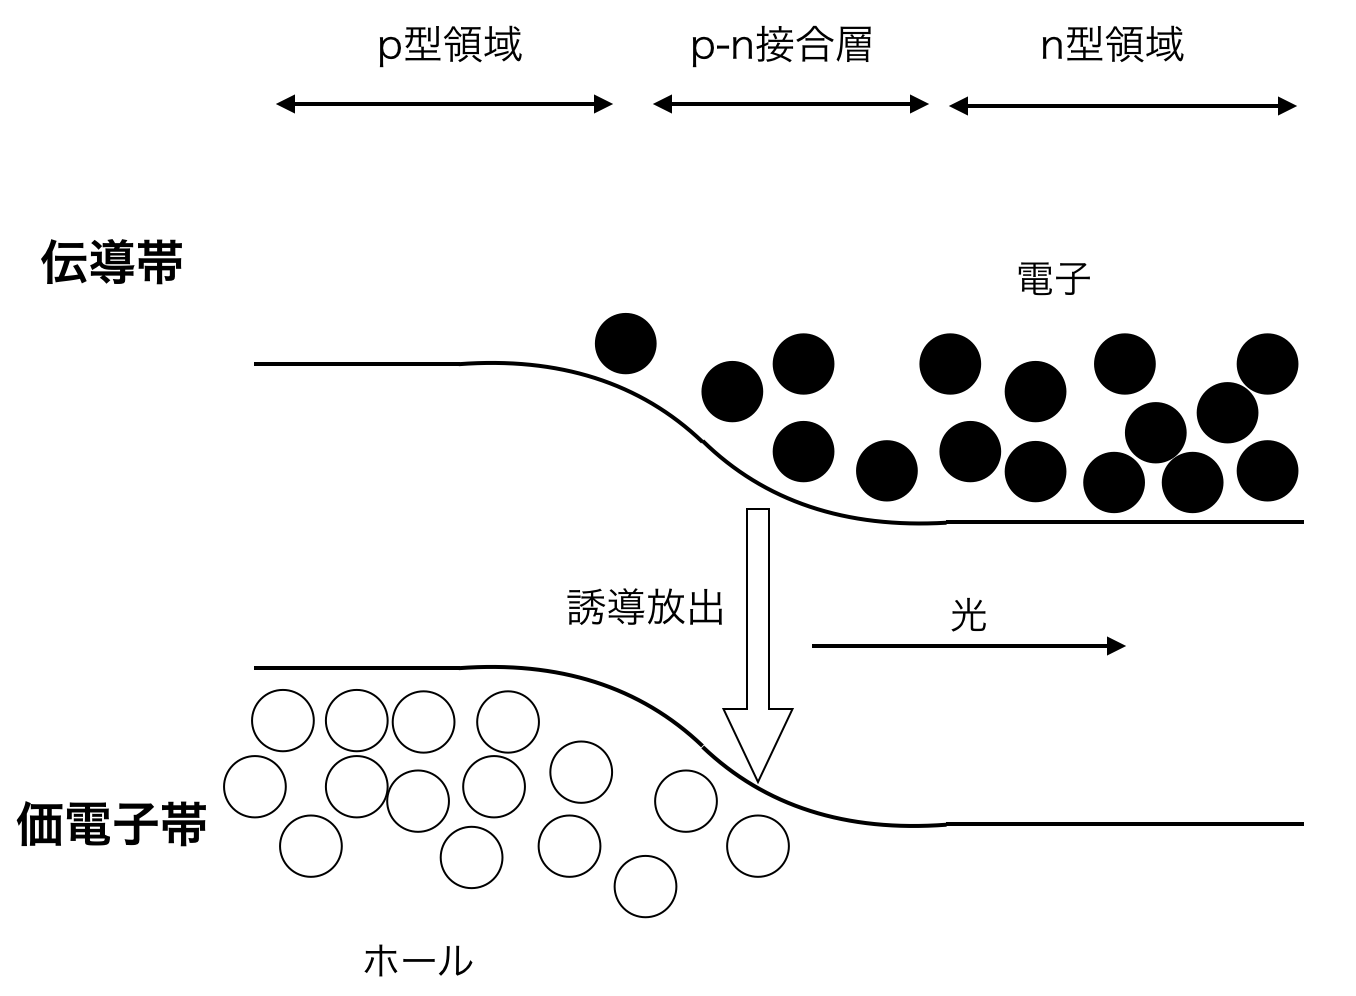
\includegraphics[keepaspectratio,  scale=0.30,  angle=0]
                          {figures/chapter2/semicon_bands.png}
                          \caption{半導体レーザーのバンド図}
                          \label{semicon_bands}
      \end{minipage}

  \end{tabular}
\end{figure}
\newpage

\subsection{テーパーアンプ}
 TAは近赤外の連続波(continuous wave,  cw)のレーザーを$20$ dB以上の利得で増幅することができる素子として知られている\cite{Cruz:06}.\\
 TAは図\ref{TA_structure}のような構造をしており, 半導体レーザーと同じDH構造を有している. TAの特徴は入力側から出力側にだんだんと拡がっているゲイン領域である. また, 増幅器として用いるためへき界面に反射材がコーティングされておらず光フィードバックがないことが半導体レーザーとの大きな違いである.\\
 TAの一つの特徴は従来の細いストライプを持つ半導体レーザーよりも高い輝度を出せることである. 輝度は
 \begin{equation}
   B = P/(A\Omega)
 \end{equation}
で定義される. ただし, Pは光の出力パワー, Aは放出面積, $\Omega$は光の放出される立体角を表す. 輝度は, レーザーの空間モードが一つであるとき, およそ
\begin{equation}
  B = P/\lambda^2
\end{equation}
の最大値をとる\cite{Walpole1996}. ただし, $\lambda$は波長を表す. このようなレーザーのビームを回折限界であるという. 従来の幅の細いゲイン領域ではバルクや発光面の加熱効果によって得られるパワーが数百ミリワットに限られていた. また, より幅のあるゲイン領域を用いると横モードを一つに保つことが難しいという欠点があった.これに対して, cwレーザーをTAを用いて増幅した場合, 数ワットの回折限界の出力を得ることができる\cite{Walpole1996}.


\begin{figure}[htbp]
 \begin{center}
  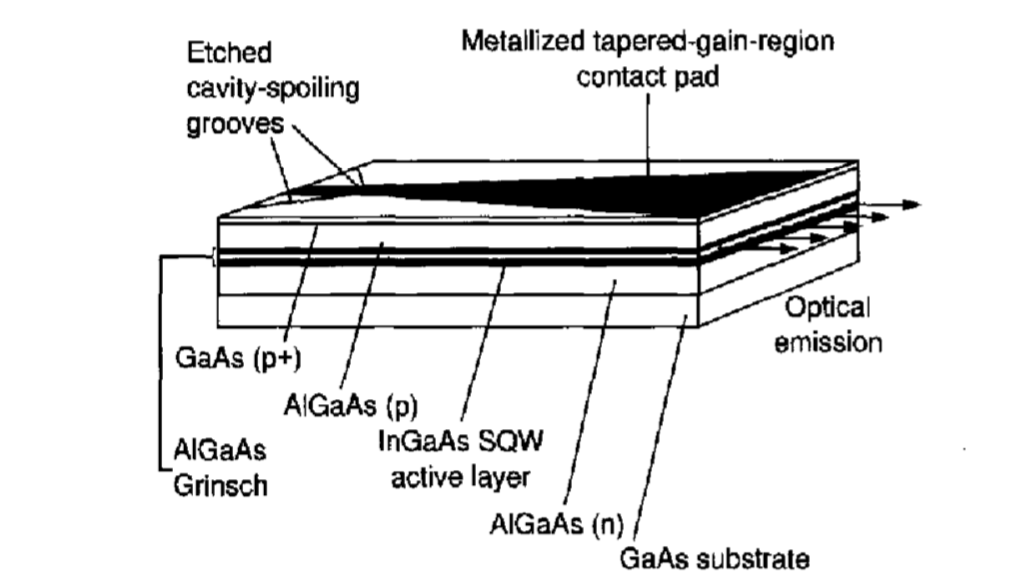
\includegraphics[width=100mm]{figures/chapter2/TA_structure.png}
 \end{center}
 \caption{TAの基本構造(文献\cite{Walpole1996}から引用)}
 \label{TA_structure}
\end{figure}

\newpage
\chapter{過去の研究に基づくCs原子の二光子冷却のシミュレーション}
\section{従来の課題と光周波数コムによる冷却のメリット}

 従来のレーザー冷却では, アルカリ金属やアルカリ土類金属などの限られた原子しか冷却できなかった.この理由としては主に2つの理由が挙げられる. 1つ目としては, 水素や酸素を含む多くの原子の遷移エネルギーは真空紫外領域に相当しており現在はこの領域で十分な強度のレーザーを得ることができていないことがある. 2つ目は, 多くの原子ではエネルギー準位の構造が複雑であり励起された原子が準安定な準位に緩和してしまうので, これを励起するためのレーザーを用意する必要があり実験の系が複雑化してしまうことである\cite{PhysRevA.73.063407}.\\
 光周波数コムを用いた二光子のレーザー冷却は, 2006年にKielpinski氏らによって提案された\cite{PhysRevA.73.063407}. 光周波数コムを用いることにより, 上記の2つの課題を克服することができる. まず, 光周波数コムは高強度のピークパワーをもつため, 同じ時間平均パワーをもつcwレーザーに比べて高効率の非線形光学効果を利用することができ, より高強度の短波長のレーザーを得ることができる. また, 光周波数コムの複数の縦モードをリポンプレーザーとして利用できるために, 実験の系を簡単にすることができる. これらの長所により, 光周波数コムはcwレーザーよりも効率の良い二光子冷却を実現することができると期待される\cite{PhysRevA.73.063407}.\\
 本章では, コムを用いた二光子冷却についての過去の研究の内容を紹介する.

\section{二光子コムによるレーザー冷却の理論}
 Jayichらの論文\cite{PhysRevX.6.041004}で説明されている, 二光子遷移を用いた光周波数コムレーザー冷却の理論を紹介する.\\
コムによる二光子の遷移を考えるとき, パルスに含まれる二光子のエネルギーもまた, コム(櫛)を形成する.これを二光子コムと呼ぶことにすると, 二光子コムのn番目の縦モードの周波数は
\begin{equation}
f_n = nf_r + 2f_0
\end{equation}
となる. ただし, $f_r$:は繰り返し周波数, $f_0$はキャリアエンベロープオフセット周波数を表す. モード同期レーザーについては実効的な共鳴ラビ周波数を求めることができる. 二光子コムのn番目のコムの歯共鳴ラビ周波数は,
\begin{eqnarray}\label{ResonanceRabi}
\Omega _{n} &=&\sum _{p}\frac {g^{\left( 1\right) }_{p}g^{\left( 2\right) }_{n-p}}{2\Delta_p} \nonumber\\
&=& \sum _ { p } \frac { e ^ { 2 } \mathcal { E } _ { p } \mathcal { E } _ { n - p } } { \hbar ^ { 2 } } \left\langle \mathrm { e } \left| ( \hat { \boldsymbol { \epsilon } } \cdot \mathbf { r } ) \left( \sum _ { \mathrm { i } } \frac { | \mathrm { i } \rangle \langle \mathrm { i } | } { 2 \Delta _ { p } ^ { ( \mathrm { i } ) } } \right) ( \hat { \boldsymbol { \epsilon } } \cdot \mathbf { r } ) \right| \mathrm { g } \right\rangle
\end{eqnarray}\\
ただし, $g^{\left( 1\right) }_{p}$は$p$番目のコムの歯による基底状態から中間状態への共鳴一光子ラビ周波数, $g^{\left( 2\right) }_{p}$は$p$番目のコムの歯による中間状態から励起状態への共鳴一光子ラビ周波数を表す.
$\Delta _{p}=pf_{r}+f_{0}-f_{gi}$は一光子の中間状態からの離調である. ただし, $f_{gi}$は基底状態から中間状態へのエネルギー差をプランク定数$h$で割ったものである.また、$\epsilon_0$は真空の誘電率、$c$は光速、$e$は電気素量、$\hbar$はプランク定数$h$を$2\pi$で割った値を表す。\\
二光子コムのN番目のコムの歯が共鳴周波数に最も近いとき, 速度$v$で動く原子の励起確率の時間平均は,
\begin{equation}\label{ExcitationRate}
\gamma_\mathrm{comb} = \frac{\Omega^2_{N}T_\mathrm{r}} {4} \frac{\sinh(\gamma T_\mathrm{r}/2)}{\cosh(\gamma T_\mathrm{r}/2) - \cos(\delta_N(\bm{v})T_\mathrm{r})}
\end{equation}
ここで, $\delta _{N}\left( v\right) \equiv 2\pi ( f_\mathrm{\mu }-f_\mathrm{ge}-f_{N}\widehat {\bm{k}}\cdot {\bm{v}}/c )$は$N$番目の二光子コムの歯の共鳴周波数からの離調を表す.$f_{ge}$は励起状態と基底状態のエネルギー差をプランク定数で割ったもの, $\widehat {\bm{k}}$はレーザーの進行方向の単位ベクトル, $\gamma$は励起準位の自然幅を表す.\\
離調$\delta _{N}\left( v\right)$と自然幅$\gamma$の両方がコムの歯の間隔($2\pi f_r$)よりも小さいとき, 二光子コムは二光子ラビ周波数$\Omega_N$の一つの縦モードとして扱うことができる.この近似の下では, 励起確率は
\begin{equation}\label{EffectiveExcitationRate}
\gamma_N = \frac{\Omega^2_N}{\gamma}\frac{1}{1 + [2\delta_N(\bm{v})/\gamma]^2}
\end{equation}
と表せる.\\
 また, (二色のコムによる冷却ではなく)縮退したコムによる二光子冷却の場合, ドップラー冷却限界温度は
\begin{equation}
  T_\mathrm{D} = \frac{3}{4}\frac{\hbar\gamma}{2k_\mathrm{B}}
\end{equation}
となることが分かっている. ただし, $k_\mathrm{B}$はボルツマン定数である。\\
 Jayichらの論文\cite{PhysRevX.6.041004}では, 初めて光周波数コムを用いた二光子冷却の実証実験が行われた.Jayichらのグループはルビジウムの縮退した二光子のコムによる一次元のレーザー冷却に成功し, $57 \mathrm{\mu K}$を達成している.

\section{Cs原子の冷却に必要な励起効率の見積もり}
  今回はあらかじめMOTで予冷されたCs原子を冷却することを目指すが、その際に必要な二光子遷移の励起効率を見積もる。$6 ^ { 2 } S _ { 1 / 2 }$の$F = 4$から$6 ^ { 2 } P _ { 3 / 2 }$の$F ^ { \prime } = 5$の遷移によるドップラー冷却を行った場合、ドップラー冷却温度は$125.61\ \mathrm{\mu K}$となる\cite{Cs_level_diagram}。このことから、二光子コム照射時のCs原子の温度は数百$\mathrm{\mu K}$以下にできると考えられる。原子の温度が$T$ Kのときの原子の速さの最頻値は
\begin{equation}
  v _ { \mathrm { th } } = \sqrt { \frac { 2 k _ { \mathrm { B } } T } { m }}
\end{equation}
で与えられる。ただし、mは原子の質量を表す。MOT後の原子の速さはこの最頻値を持つものとして計算する。例えば、$126\ \mathrm{\mu K}$のCs原子の速さの最頻値は$125$ mm/sである。また6s軌道から8s軌道への二光子遷移を利用して冷却する場合、二つの光子の周波数が同じであるとすると822nm程度の波長を持つ。この場合二光子を吸収した時のCs原子の速度変化は二光子を吸収するごとに$7.3$ mm/s程度の減速である。
ドップラー冷却における加熱効果を無視して、近似的に原子が等加速度$a\ \mathrm{m/s^2}$で減速するとすると、速度$v$を持つ原子が停止するまでに移動する距離$l$は
\begin{equation}
    l = \frac{v^2}{2a}
\end{equation}
で与えられる。実験で用いるレーザーの直径を考慮して原子が冷却されるまでに$0.5$ mm以内の移動距離に抑えるのに必要な加速度から冷却に必要な励起効率を初期温度に応じて計算すると、図\ref{necessary_excitation_rate}のようになる。この結果と実験上のロスを考慮して今回の実験では$10000\ \mathrm{s^{-1}}$の励起効率を目標とする。
\begin{figure}[htpb]
  \centering
    \begin{tabular}{c}
      \begin{minipage}{1\hsize}
        \centering
          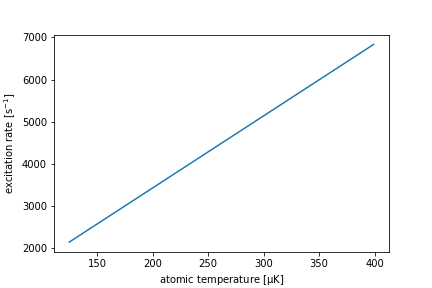
\includegraphics[keepaspectratio,  scale=0.6,  angle=0]
                          {figures/chapter3/necessary_excitation_rate.png}
                          \caption{MOTで予冷したCs原子の冷却に必要な励起効率。計算の詳細については本文中に記載。}
                          \label{necessary_excitation_rate}

      \end{minipage}
    \end{tabular}
\end{figure}
\section{Cs原子の二色のコムによる励起効率の見積もり}
 Jayichらの論文\cite{PhysRevX.6.041004}では、Rb原子の5s軌道から5d軌道への遷移を利用しており、以下のパラメータの下で実験を行っている。
\begin{itemize}
  \item 5d順位の線幅 : $2\pi \times 667$ kHz
  \item コムのパルス幅 : $2-5$ ps
  \item コムの平均パワー : $500$ mW
  \item コムビームの直径 : $1$ mm
  \item コムの周波数帯域 : $500$ GHz
  \item コムの繰り返し周波数 : $80$ MHz
\end{itemize}
Jayichらはこのパラメータの下で励起効率を$\gamma_N \sim 13000\ \mathrm{s^{-1}}$と見積もっている。\\
 Jayichらの論文\cite{PhysRevX.6.041004}の励起確率の計算手法に習い、今回私達の用いるコムでCs原子を冷却する際の励起確率の計算を行った。その計算に際して以下の五つの近似を行った。\\
\\
 (a) $\delta_N(\bm{v}) = 0$とし、
\begin{equation}
  \gamma_N = \frac{\Omega^2_N}{\gamma}
\end{equation}
     とした。\\
 (b) 二光子励起の際の中間状態として$6P_{\frac{3}{2}}$以外の状態を無視した。\\
 (c) 光周波数コムの全ての縦モードの電場の強さが一定であるとして計算を行った。
\begin{equation}
  \mathcal{E}_p = const.
\end{equation}
 (d) 以下の関係式を用いた。
\begin{equation}
  \Sigma_{p} \mathcal{E}_p\mathcal{E}_{n-p} \approx 2I/\epsilon_0 c
\end{equation}
 (e) $\left\langle \mathrm { e } \left| ( \hat { \boldsymbol { \epsilon } } \cdot \mathbf { r } ) | \mathrm { i } \rangle \langle \mathrm { i } |  ( \hat { \boldsymbol { \epsilon } } \cdot \mathbf { r } ) \right| \mathrm { g } \right\rangle$ の値がCs原子とRb原子で等しいとした。\\
\\
 (a)-(d)の近似を用いると、励起効率の式(\ref{EffectiveExcitationRate})は以下のように計算できる。\\
\begin{eqnarray}\label{approx_ex-rate}
  \gamma_N &=& \frac{\Omega^2_N}{\gamma}\frac{1}{1 + [2\delta_N(\bm{v})/\gamma]^2} \nonumber\\
  &=& \frac{\Omega^2_N}{\gamma}  \nonumber\\
  &=& \frac{1}{\gamma} \Biggl[ \sum _ { p } \frac { e ^ { 2 } \mathcal { E } ^{(1)}_ { p } \mathcal { E }^{(2)} _ { N - p } } { \hbar ^ { 2 } } \left\langle \mathrm { e } \left| ( \hat { \boldsymbol { \epsilon } } \cdot \mathbf { r } ) \left(  \frac { | \mathrm { i } \rangle \langle \mathrm { i } | } { 2 \Delta _ { p } ^ { ( \mathrm { i } ) } } \right) ( \hat { \boldsymbol { \epsilon } } \cdot \mathbf { r } ) \right| \mathrm { g } \right\rangle \Biggr]^2 \nonumber \\
  &=& \frac{1}{\gamma} \Biggl[ \sum _ { p } \frac { e ^ { 2 } \mathcal { E }^{(1)} \mathcal { E } ^ {(2)} } { \hbar ^ { 2 } } \left\langle \mathrm { e } \left| ( \hat { \boldsymbol { \epsilon } } \cdot \mathbf { r } ) \left(  \frac { | \mathrm { i } \rangle \langle \mathrm { i } | } { 2 \Delta _ { p } ^ { ( \mathrm { i } ) } } \right) ( \hat { \boldsymbol { \epsilon } } \cdot \mathbf { r } ) \right| \mathrm { g } \right\rangle \Biggr]^2 \nonumber \\
  &=& \frac{e^2  \mathcal { E } ^ {(1)} \mathcal { E } ^ {(2)}}{ 2 \gamma \hbar ^ { 2 }  }\Biggl[ \left\langle \mathrm { e } \left| ( \hat { \boldsymbol { \epsilon } } \cdot \mathbf { r } ) | \mathrm { i } \rangle \langle \mathrm { i } |  ( \hat { \boldsymbol { \epsilon } } \cdot \mathbf { r } ) \right| \mathrm { g } \right\rangle\sum _ { p }\frac{1}{2 \Delta _ { p } ^ { ( \mathrm { i } ) }} \Biggr]^2\\
  \mathcal{E}^{(i)} &=&  \sqrt{\frac{2 I_{i}}{M \epsilon_0 c}}\ \ \ \ (i = 1,2)
\end{eqnarray}\\
ただし、$\mathcal{E}^{(1)}_p$は基底状態から中間状態へのコムの$p$番目の縦モードの電場の大きさを表し、、$\mathcal{E}^{(2)}_p$は中間状態から励起状態へのコムの$p$番目の縦モードの電場の大きさを表す。$\mathcal{E}^{(i)}\ \ (i = 1,2)$は近似(c)の下でのコムの電場の強さを表す。$I_{i}\ \ (i = 1,2)$はそれぞれのコムの強度を表す。$M$はコムの歯の本数を表し、計算上では2つのコムの歯の数は等しいとした。\\
 まず、Jayichらのグループが計算で得た励起効率から計算すると
\begin{equation}
\left\langle \mathrm { e } \left| ( \hat { \boldsymbol { \epsilon } } \cdot \mathbf { r } ) | \mathrm { i } \rangle \langle \mathrm { i } |  ( \hat { \boldsymbol { \epsilon } } \cdot \mathbf { r } ) \right| \mathrm { g } \right\rangle = 4.1 \times 10^{-22} \mathrm{m^2}
\end{equation}
を得る。この値をCsでも用いて計算する。\\
 今回の実験ではCsの$6S_{1/2}$から$8S_{1/2}$の二光子遷移を利用して冷却を行う。まず、中心波長$822$ nmの同じコムから二光子を吸収した場合での励起効率の計算を行った。このときのパラメータを以下に示す。
\begin{itemize}
  \item 遷移 : $6S_{1/2}$から$8S_{1/2}$
  \item 8S順位の線幅 : $2\pi \times 2.18$ MHz
  \item コムビームの直径 : $1$ mm
  \item コムの周波数帯域 : $20$ THz
  \item コムの繰り返し周波数 : $120$ MHz
  \item 中間状態の$6P_{\frac{3}{2}}$への遷移周波数は852nmとする。
\end{itemize}
以上の条件の下で、式(\ref{approx_ex-rate})を用いて二光子励起効率のコムのパワー依存性を計算すると図\ref{degenerated_2_photon_excitation_rate-P}のようになる。このグラフから、励起効率が不足していることが分かる。\\
\begin{figure}[htpb]
  \centering
    \begin{tabular}{c}
      \begin{minipage}{1\hsize}
        \centering
          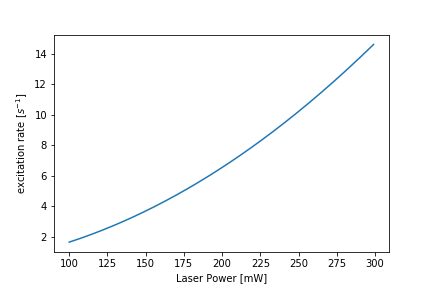
\includegraphics[keepaspectratio,  scale=0.6,  angle=0]
                          {figures/chapter3/degenerated_2_photon_excitation_rate-P.png}
                          \caption{縮退した二光子で冷却した場合の励起効率。計算の詳細は本文中に記載。}
                          \label{degenerated_2_photon_excitation_rate-P}
      \end{minipage}
    \end{tabular}
\end{figure}


\section{二色のコムによる励起に必要なパワーの見積もり}
\subsection{一光子遷移による中間状態への励起効率の見積もり}
 上述のシミュレーションで励起効率が低下した要因としては、中間状態である$6P_{\frac{3}{2}}$からの一光子コムの離調が大きいことが挙げられる。このことから、周波数の異なる二つの光子による励起により中間状態からの一光子コムの離調を小さくすることで励起効率を向上させることができるのではないかと考えられる。しかし、二色のコムで冷却する場合は一光子コムの歯と中間状態の離調をどの程度まで小さくできるかについても注意する必要がある。なぜなら、あまりに離調を小さくしすぎると中間状態に電子が励起される一光子励起の過程が支配的になってしまうからである。離調をどの程度まで小さくできるかについては一光子の散乱効率を評価することで判断した。二光子冷却時のレーザーの照射時間は、Jayichらの論文での冷却時間を参考にして5msであると仮定する。このレーザーの照射時間における一光子の散乱回数が$1$以下になることを期待すると、散乱効率は$200\ \mathrm{s^{-1}}$以下である必要がある。\\
 散乱効率は次の式で与えられる。
\begin{equation}
  R _ { \text { scatt } } = \frac { \Gamma } { 2 } \frac { \Omega ^ { 2 } / 2 } { \delta ^ { 2 } + \Omega ^ { 2 } / 2 + \Gamma ^ { 2 } / 4 }
\end{equation}
この式は飽和パラメーター$s$を用いて
\begin{equation}
  R _ { \text { scatt } } = \frac { \Gamma } { 2 } \frac{s}{1+s}
\end{equation}
と表せる。$s$は吸収遷移の飽和強度$I_0$と用いるレーザーの強度$I$により、
\begin{equation}
  s = \frac{I/I_0}{1+(2\delta/\Gamma)^2}
\end{equation}
と書けるのでこれを用いて計算する\cite{ノーベル賞と分光学}。なお、予めMOTで冷却済みのためドップラー効果の寄与は無視した。Cs原子の中間状態は$6P_{\frac{1}{2}}$($\Gamma = 4.56$ MHz,\ $I_0 = 2.50 \mathrm{\ mW/cm^2}$)を用いた\cite{CsDLine}。また、強度については近似 (c)を用いて、全体の強度をコムの歯の数で割ったものを一本のコムの歯の強度として、全てのコムの歯における$R _ { \text { scatt } }$を独立に計算し、その総和をコム全体の$R _ { \text { scatt } }$とした。この際の、コムの周波数幅は$6S_{\frac{1}{2}}$から$6P_{\frac{1}{2}}$
の共鳴周波数付近で$10$ nm程度の波長幅に対応する$5$ THzとした。繰り返し周波数$f_{\mathrm{rep}}$については当実験室にある二種類のコムの繰り返し周波数である$120$ MHzと$1.6$ GHzにおいて計算を行った。その結果を示したのが図\ref{1photon-sc-rate-2dcolor_120MHz_log},\ref{1photon-sc-rate-2dcolor_16GHz_log}である。\\
\begin{figure}[H]
  \centering
    \begin{tabular}{c}
      \begin{minipage}{1\hsize}
        \centering
          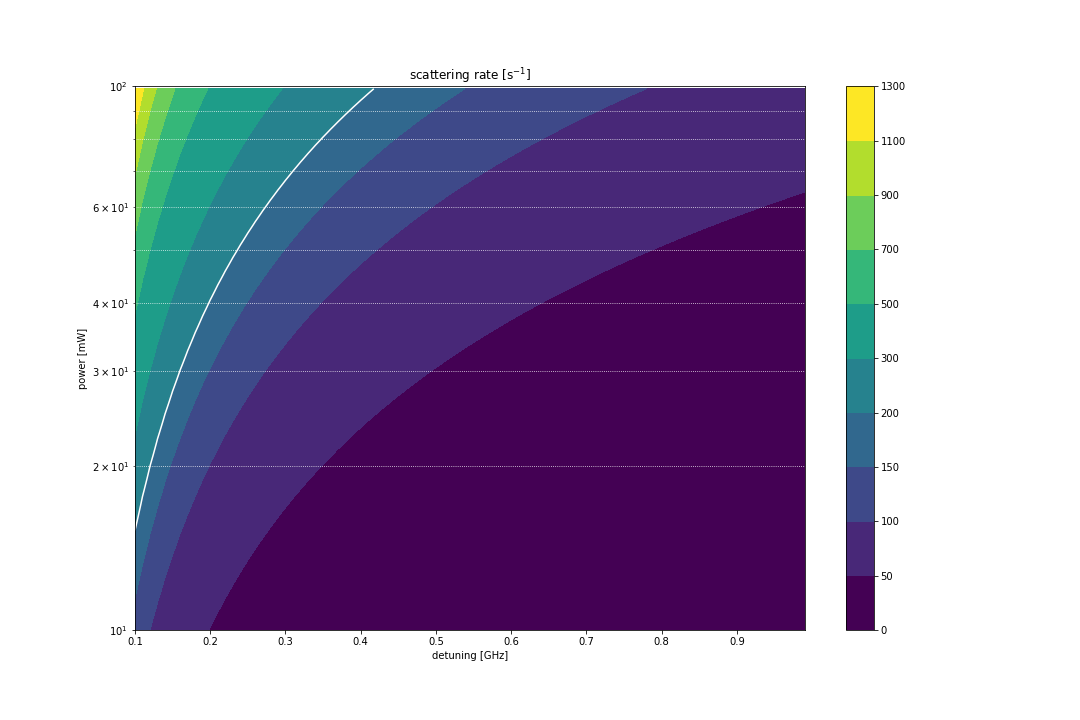
\includegraphics[keepaspectratio,  scale=0.35,  angle=0]
                          {figures/chapter3/1photon-sc-rate-2dcolor_120MHz_log.png}
                          \caption{中間状態への励起効率の離調とパワー依存性。横軸は$6S_{\frac{1}{2}}$から$6P_{\frac{1}{2}}$の共鳴にもっとも近い一光子コムの歯と$6P_{\frac{1}{2}}$の離調を示している。コムの周波数幅は$5$ THz, $f_{\mathrm{rep}}$は$120$ MHzとしている。グラフ中の白い実線が励起効率$200\ \mathrm{s^{-1}}$を表す。}
                          \label{1photon-sc-rate-2dcolor_120MHz_log}
      \end{minipage}\\
      \begin{minipage}{1\hsize}
        \centering
          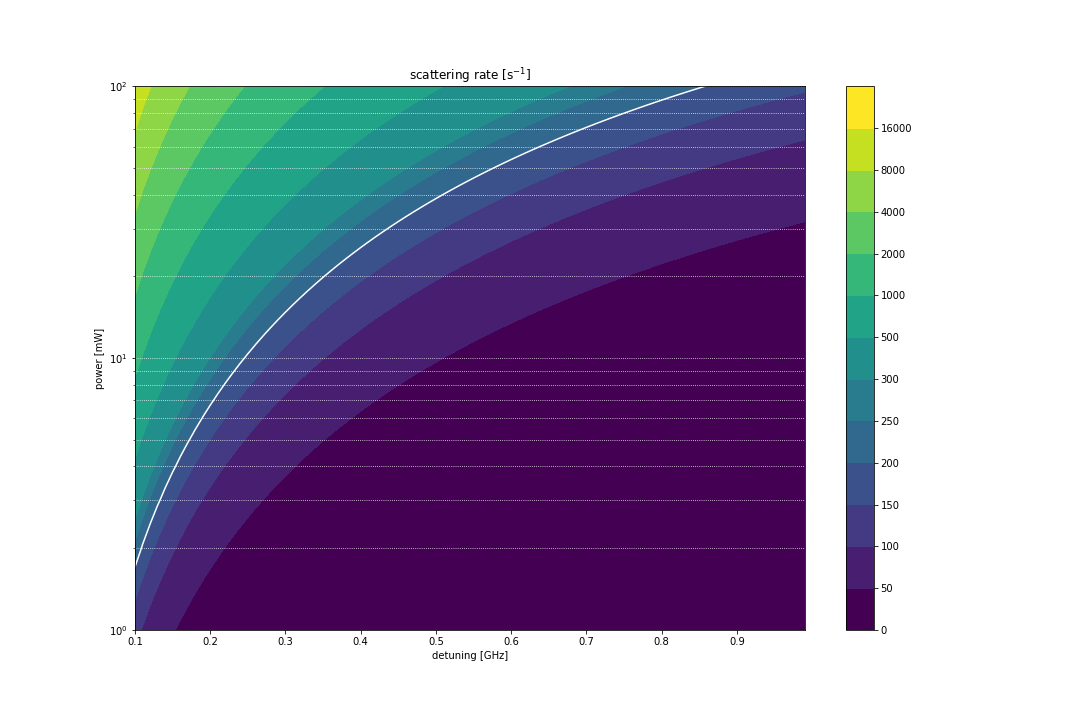
\includegraphics[keepaspectratio,  scale=0.35,  angle=0]
                          {figures/chapter3/1photon-sc-rate-2dcolor_16GHz_log.png}
                          \caption{中間状態への励起効率の離調とパワーの依存性。横軸は$6S_{\frac{1}{2}}$から$6P_{\frac{1}{2}}$の共鳴にもっとも近い一光子コムの歯と$6P_{\frac{1}{2}}$の離調を示している。コムの周波数幅は$5$ THz, $f_{\mathrm{rep}}$は$1.6$ GHzとしている。グラフ中の白い実線が励起効率$200\
                          \mathrm{s^{-1}}$を表す。}
                          \label{1photon-sc-rate-2dcolor_16GHz_log}
      \end{minipage}
    \end{tabular}
\end{figure}
\newpage
\subsection{二色のコムによる冷却に必要なパワーの見積もり}
このように波長の異なるコムを用意するには、周波数幅の広いコムからバンドパスフィルター(BPF)を用いて目的の周波数帯を取り出す必要がある。しかし、単に切り出すだけでは光のパワーが低下してしまい励起効率が低下することが予想される。そのため、二色のコムを用いて励起する場合二色のどのような強度のコムを用意すると目標の励起効率が得られるのかのシミュレーションを行った。その際前節の議論を踏まえ、$f_{\mathrm{rep}} = 120$ MHzのコムでは、$6P_{\frac{1}{2}}$と最近接の一光子コムの歯の離調が$200$ MHz, $400$ MHzの際の励起効率を二つのコムのパワーに応じて計算した。この際、一光子の$6P_{\frac{1}{2}}$への散乱効率が$1 \mathrm{s^{-1}}$よりも大きくならないように注意して、$894$ nm側のコムのパワーを設定した。計算の結果を図\ref{5THz-120MHz-04GHz_new}, \ref{5THz-120MHz-02GHz_new}, \ref{5THz-16GHz-04GHz_new}, \ref{5THz-16GHz-08GHz_new}に示す。この計算結果から$10000 \mathrm{s^{-1}}$の励起効率を得るために、必要な二色のコムのパワーと中間状態からの一光子コムの歯の離調のおよその組み合わせを見積もることができた。\\
\newpage
\begin{figure}[H]
  \centering
    \begin{tabular}{c}
      \begin{minipage}{1\hsize}
        \centering
          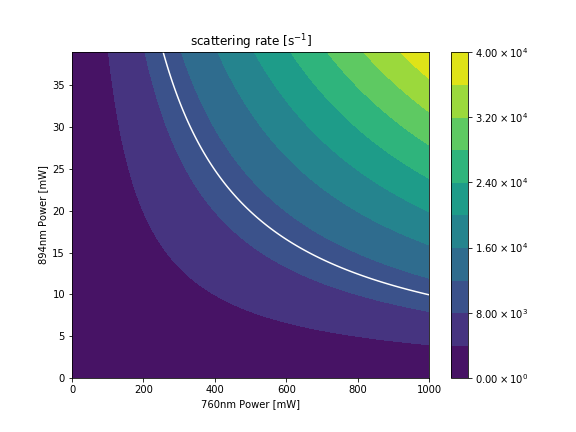
\includegraphics[keepaspectratio,  scale=0.6,  angle=0]
                          {figures/chapter3/2dcolor/5THz-120MHz-02GHz_new.png}
                          \caption{$f_\mathrm{rep} = 120\ \mathrm{MHz}$で$6P_{\frac{1}{2}}$と最近接の一光子コムの歯の離調が$200$ MHzのときの、二光子励起効率のパワー依存性。図中の白い実線が$10000\ \mathrm{s^{-1}}$の励起効率を示す。}
                          \label{5THz-120MHz-02GHz_new}
      \end{minipage}\\
      \begin{minipage}{1\hsize}
          \centering
            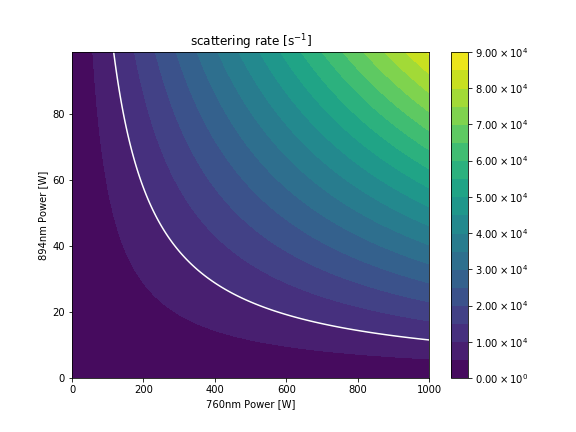
\includegraphics[keepaspectratio,  scale=0.6,  angle=0]
                            {figures/chapter3/2dcolor/5THz-120MHz-04GHz_new.png}
                            \caption{$f_\mathrm{rep} = 120\ \mathrm{MHz}$で$6P_{\frac{1}{2}}$と最近接の一光子コムの歯の離調が$400$ MHzのときの、二光子励起効率のパワー依存性。図中の白い実線が$10000\ \mathrm{s^{-1}}$の励起効率を示す。}
                            \label{5THz-120MHz-04GHz_new}
        \end{minipage}
    \end{tabular}
\end{figure}

\begin{figure}[H]
  \centering
    \begin{tabular}{c}
      \begin{minipage}{1\hsize}
        \centering
          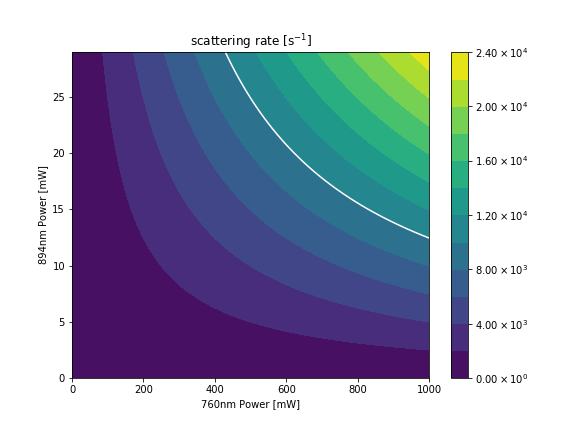
\includegraphics[keepaspectratio,  scale=0.6,  angle=0]
                          {figures/chapter3/2dcolor/5THz-16GHz-04GHz_new.png}
                          \caption{$f_\mathrm{rep} = 1.6\ \mathrm{GHz}$で$6P_{\frac{1}{2}}$と最近接の一光子コムの歯の離調が$400$ MHzのときの、二光子励起効率のパワー依存性。図中の白い実線が$10000\ \mathrm{s^{-1}}$の励起効率を示す。}

                          \label{5THz-16GHz-04GHz_new}
      \end{minipage}\\
        \begin{minipage}{1\hsize}
          \centering
            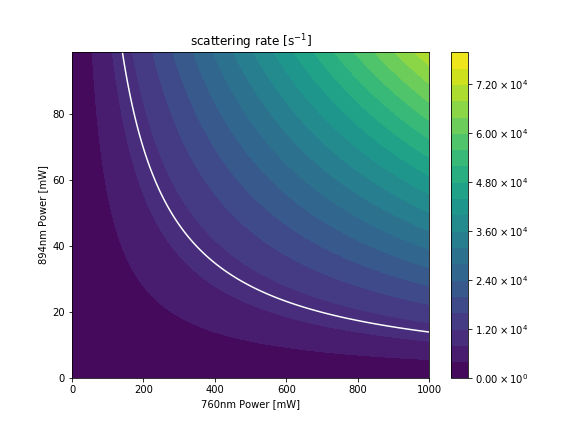
\includegraphics[keepaspectratio,  scale=0.6,  angle=0]
                            {figures/chapter3/2dcolor/5THz-16GHz-08GHz_new.png}
                            \caption{$f_\mathrm{rep} = 1.6\ \mathrm{GHz}$で$6P_{\frac{1}{2}}$と最近接の一光子コムの歯の離調が$800$ MHzのときの、二光子励起効率のパワー依存性。図中の白い実線が$10000\ \mathrm{s^{-1}}$の励起効率を示す。}
                            \label{5THz-16GHz-08GHz_new}
        \end{minipage}
    \end{tabular}
\end{figure}

\begin{comment}
\newpage
  実験系の以下のパラメータを用いて二色のコムでの励起効率の計算を行った。
\begin{itemize}
  \item 遷移 : 6sから8s
  \item 8S順位の線幅 : $2\pi \times 2.18$ MHz
  \item レーザービームの直径 : $0.5$ mm
  \item 760nm付近の波長を持つコムの強度 : $1$ W
  \item 894nm付近の波長を持つコムの強度 : $10$ mW
  \item コムの繰り返し周波数 : $1.6$ GHz
  \item 中間状態にもっとも近い二光子コムの歯の$6P_{\frac{3}{2}}$からの離調が$2 \mathrm{GHz}$
\end{itemize}
 この条件で一光子コムの周波数幅を変化させて励起効率を計算すると、図\ref{2color_excitation_rate}のようになった。切り出す周波数幅を大きくすると、中間状態からの離調が大きくなる分、励起効率が落ちることがわかる。ただし、切り出す周波数幅を小さくするとコムの強度も落ちるが、この効果は計算に取り入れられていない。

\begin{figure}[htbp]
 \begin{center}
  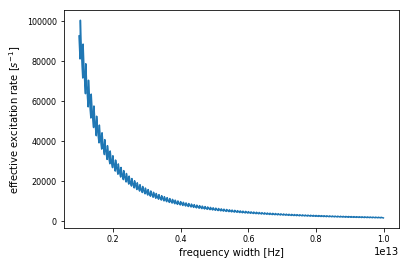
\includegraphics[width=100mm]{figures/chapter3/2color_excitation_rate_astro.png}
 \end{center}
 \caption{二光子励起効率の一光子コムの周波数幅に対する依存性}
 \label{2color_excitation_rate}
\end{figure}
\end{comment}

\chapter{Cs原子のMOTのためのcw光源の構築}
\section{飽和吸収分光法によるCs原子のロック}
\subsection{MOTに用いるCs原子の超微細構造}
 今回のMOTで用いるCs原子の準位図は図\ref{Cs_level_diagram_MOT}のようになっている。冷却に用いる遷移は$6 ^ { 2 } S _ { 1 / 2 }$の$F = 4$から$6 ^ { 2 } S _ { 3 / 2 }$の$F ^ { \prime } = 5$の遷移であるが、$6 ^ { 2 } S _ { 1 / 2 }$の$F = 3$に脱励起した電子を冷却のサイクルに戻すために$6 ^ { 2 } S _ { 1 / 2 }$の$F = 3$
から$6 ^ { 2 } S _ { 3 / 2 }$の$F ^ { \prime } = 4$の遷移に対応するレーザーも使用する。便宜的に前者のレーザーをメインレーザー、後者のレーザーをリポンプレーザーと呼ぶことにする。


\begin{figure}[htpb]
  \centering
    \begin{tabular}{c}
      \begin{minipage}{1\hsize}
        \centering
          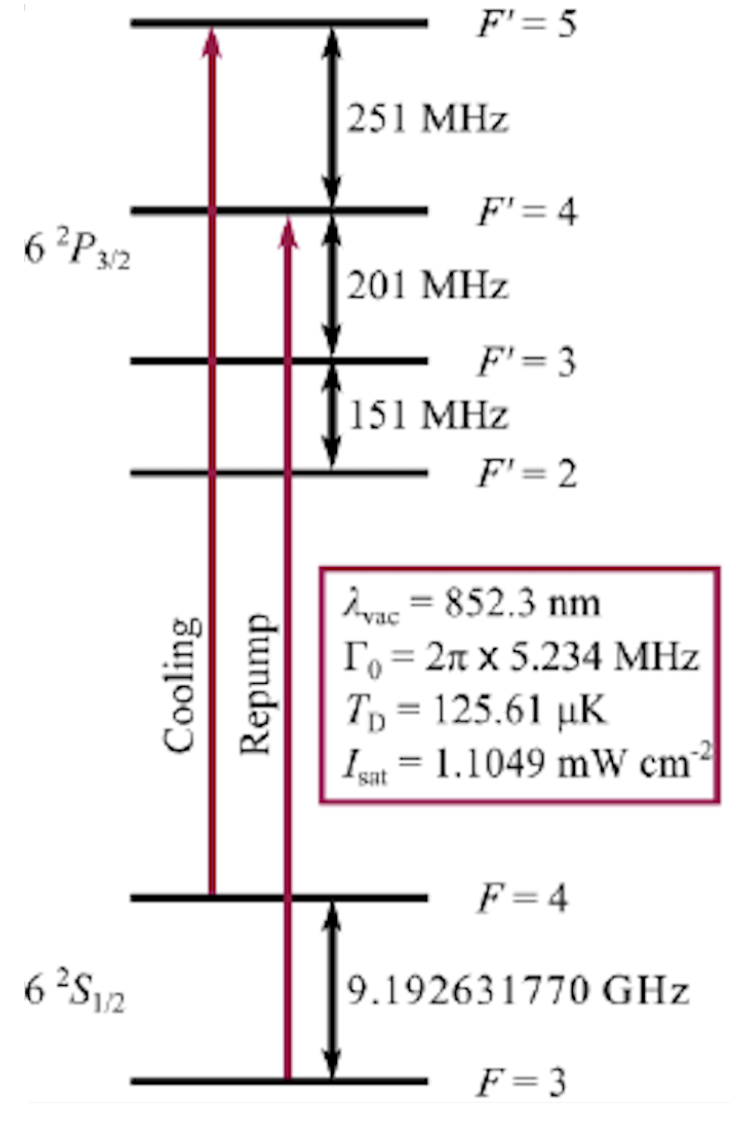
\includegraphics[keepaspectratio,  scale=0.35,  angle=0]
                          {figures/saturated-absorption/Cs_level_diagram_MOT.png}
                          \caption{MOTで用いるCs原子の超微細構造の準位図(参考文献\cite{Cs_level_diagram}から引用)}
                          \label{Cs_level_diagram_MOT}
      \end{minipage}
    \end{tabular}
\end{figure}
\subsection{ECDLによる周波数の制御}
今回の実験で飽和吸収分光に用いるためのレーザーの周波数の制御には外部共振器型半導体レーザー(External Cavity Diode Laser, ECDL)を使用している。ECDLは回折格子の持つ波長選択性を用いて特定のモードの1次回折光をレーザーダイオードに戻すことによりそのモードのゲインを上げ、他のモードのゲインを下げるというものである。この回折格子をピエゾ素子に取り付け、電気的に回折格子の角度を調整できるようにすることで目的の周波数の周辺でレーザーの周波数の挿引を可能にしている。

\begin{figure}[htpb]
  \centering
    \begin{tabular}{c}
      \begin{minipage}{1\hsize}
        \centering
          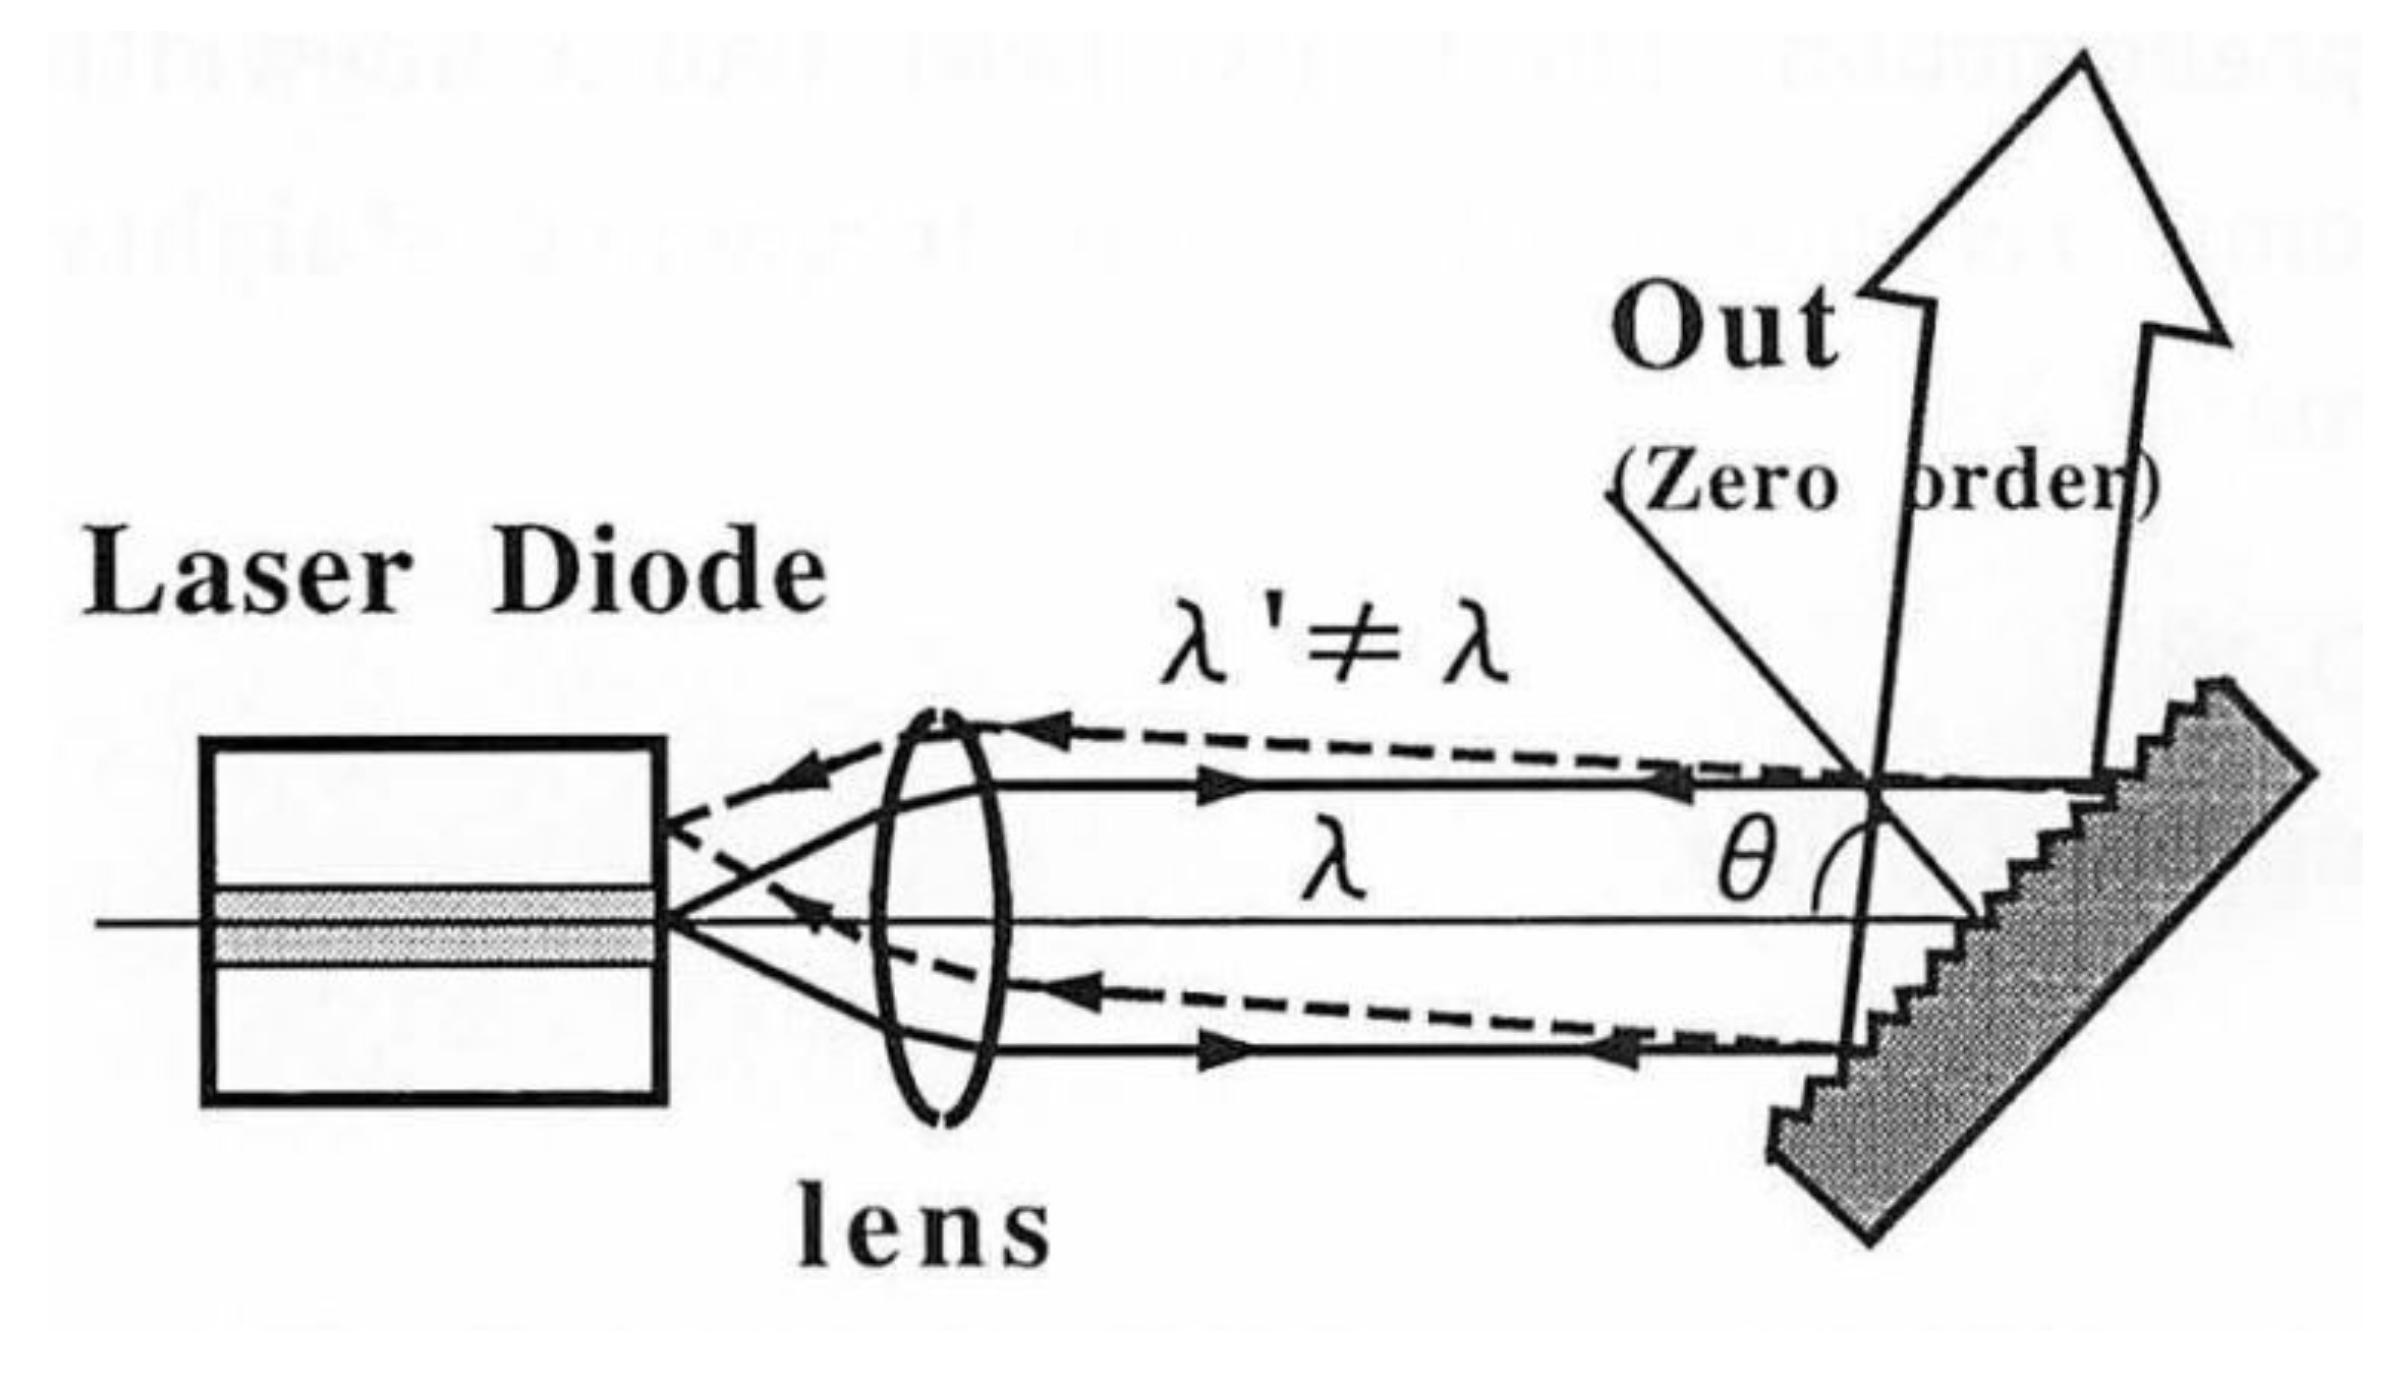
\includegraphics[keepaspectratio,  scale=0.35,  angle=0]
                          {figures/saturated-absorption/ECDL_diagram.png}
                          \caption{ECDLの概略図(参考文献\cite{ECDL}より引用)}
                          \label{ECDL_diagram}
      \end{minipage}
    \end{tabular}
\end{figure}
\subsection{FMサイドバンドロック法}
飽和吸収分光で得られたPDの信号の凹みに周波数をロックするために目的の周波数で正負が逆転するような信号(エラー信号)を生成し、フィードバックをかけることで周波数をロックするという手法を用いる。このエラー信号を生成する手法として用いるのがFMサイドバンドロック法である。この手法では、まず周波数$f_\mathrm{0}$のレーザー光の位相に対して周波数$f_\mathrm{m}$のラジオ周波数の変調を加えることで周波数空間上で元の周波数に対して周波数軸上で両側に二本の$f_\mathrm{0\pm m}$のサイドバンドを立てる。二本のサイドバンドの位相が逆であるため、それぞれのサイドバンドと元の光のヘテロダインビートを取ると、周波数の違いによるCs原子の吸収の差からエラー信号を生成する。
\subsection{今回の飽和吸収分光に用いる光学系}
 今回の実験では、メインレーザーとリポンプレーザーの飽和吸収分光を同一の気体のCs原子が入ったセルを用いて行った。そのため、光学系がやや複雑な形となったので概略図をの二つの図に分けて示した。図\ref{Main_Laser_diagram}はメインレーザーの光学系を示しているが、この光学系の外側に隣接する形で図\ref{repump_diagram}のようにリポンプレーザーの光学系を設置した。今回の実験ではピエゾ素子にファンクションジェネレーターで振動電圧を印加しレーザーの周波数を掃引している。レーザーの一部をBS(Beam Splitter)やPBS(Polarization Beam Splitter)を利用して飽和吸収分光を行い、飽和吸収分光に用いないビームをMOTに使用している。メインレーザーについてはEOM(Electro Optic Modulator)を用いて、$15$ MHz位相変調をかけることでエラー信号生成のためのサイドバンドを生成している。
\begin{figure}[H]
  \centering
    \begin{tabular}{c}
      \begin{minipage}{1\hsize}
        \centering
          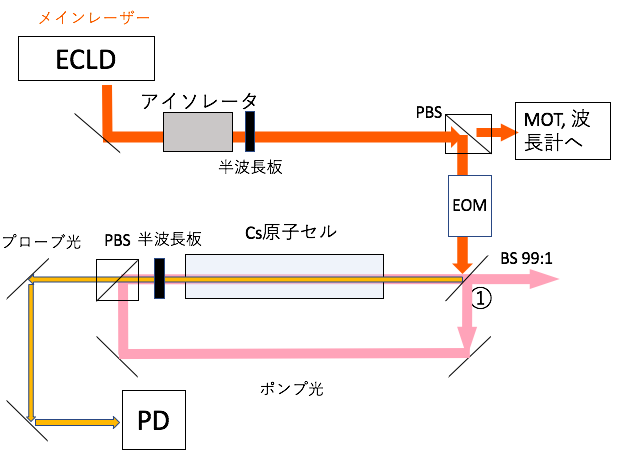
\includegraphics[keepaspectratio,  scale=0.35,  angle=0]
                          {figures/saturated-absorption/Main_Laser_diagram.png}
                          \caption{メインレーザーの光学系}
                          \label{Main_Laser_diagram}
      \end{minipage}
    \end{tabular}
\end{figure}
\begin{figure}
  \centering
    \begin{tabular}{c}
      \begin{minipage}{1\hsize}
        \centering
          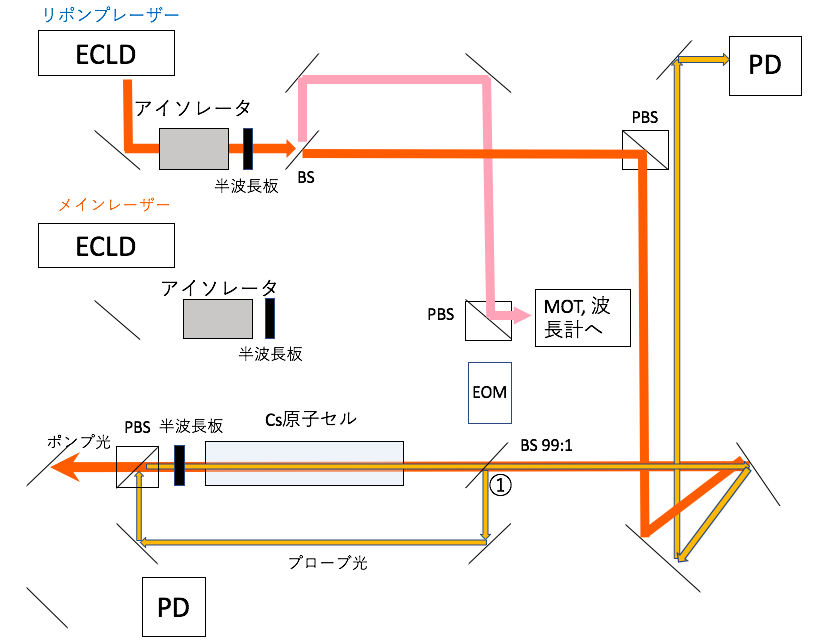
\includegraphics[keepaspectratio,  scale=0.35,  angle=0]
                          {figures/saturated-absorption/repump_diagram.png}
                          \caption{リポンプレーザーの光学系}
                          \label{repump_diagram}
      \end{minipage}
    \end{tabular}
\end{figure}
 どの遷移にロックしているかをのべる。ECDLの仕組み。ピエゾに三角波を入れて周波数の挿引を行なっていることを述べる。エラー信号の得かた。ロック回路。
\section{測定結果}
\subsection{レーザーのロック}
メインレーザーの超微細構造を捉えたPDの信号は図\ref{PD_Signal_Main}である。この時のエラーシグナルが図\ref{error_signal_main_all-structure}のようになる。図\ref{main-locking-error}は周波数ロック時のエラー信号である。これらの測定結果から周波数ロック時の線幅を評価することができる。\\
 PD信号の各極小の位置と超微細構造の対応は図のようになっている。$F_{\mathrm{e}} = 3,\ 5$のクロスオーバー共鳴の計測から$F_{\mathrm{e}} = 5$の計測までの時間$11.5$ msは$226$ MHzに対応しているため、測定時の周波数の掃引速度は$19.7$ GHz/sとなる。また、。図\ref{error_signal_main_all-structure}を見ると、$F_{\mathrm{e}} = 5$への遷移に対応する信号の変化の極小から極大への時間幅は$1.2$ msなので$F_{\mathrm{e}} = 5$
この時間幅に対応する周波数幅は$23$ MHzとなる。また電圧の極大から極小の変化は$V_{\mathrm{pp}} = 0.29$ Vなので、エラー信号の電圧と周波数の対応は$83$ MHz/Vであることが分かる。ここで図\ref{main-locking-error}に示されたロック時のエラー信号の$-0.55$ sから$-0.018$ sまでの部分の標準偏差を求めると$2.4\times 10^(-2)$ Vとなる。これに対応する周波数は$2.0$ MHzであることが分かる。このように、$F_{\mathrm{e}} = 5$の遷移に幅$2.0$ MHzでロックできていることが分かる。\\
  (ECDL自体の線幅数十-百kHzとの比較、回路の高周波ノイズがのっていると思われる)\\
 リポンプレーザーについても同様に周波数の掃引とロックを行った。図\ref{Repump_PD_signal}に実際に観測された超微細構造を示す。

\begin{figure}[b]
  \centering
    \begin{tabular}{c}

      \begin{minipage}{1\hsize}
        \centering
          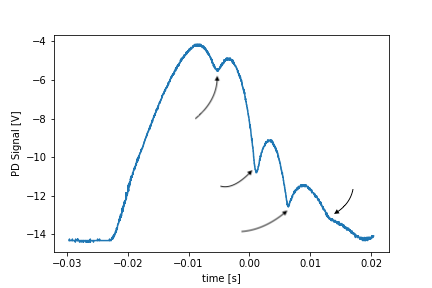
\includegraphics[keepaspectratio,  scale=0.8,  angle=0]
                          {figures/saturated-absorption/PD_Signal_Main.png}
                          \caption{PDで観測されたCs原子の超微細構造(メインレーザー)}
                          \label{PD_Signal_Main}
      \end{minipage}
  \end{tabular}
\end{figure}
\begin{figure}
  \centering
    \begin{tabular}{c}
      \begin{minipage}{1\hsize}
        \centering
          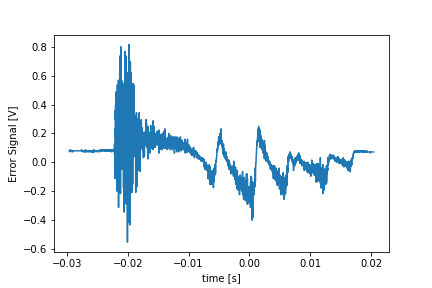
\includegraphics[keepaspectratio,  scale=0.8,  angle=0]
                          {figures/saturated-absorption/error_signal_main_all-structure.png}
                          \caption{図\ref{PD_Signal_Main}の信号のエラー信号}
                          \label{error_signal_main_all-structure}
      \end{minipage}\\

      \begin{minipage}{1\hsize}
        \centering
          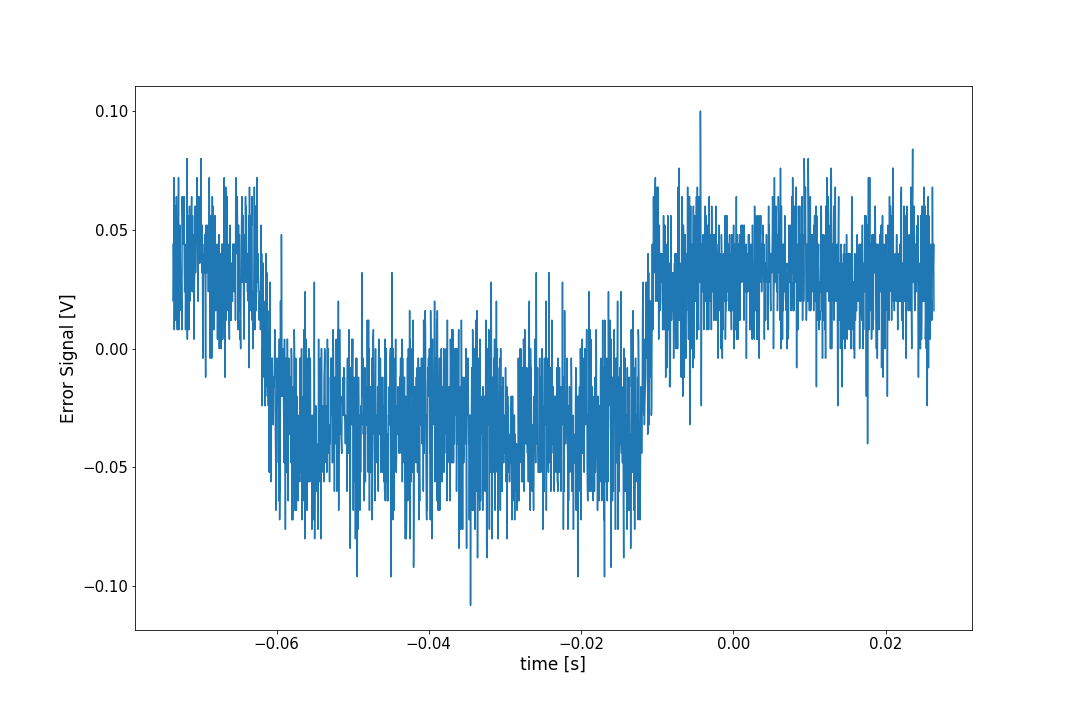
\includegraphics[keepaspectratio,  scale=0.35,  angle=0]
                          {figures/saturated-absorption/main-locking-error.png}
                          \caption{メインレーザーの周波数ロック中のエラー信号}
                          \label{main-locking-error}
      \end{minipage}
    \end{tabular}
\end{figure}

\newpage
\begin{figure}[htpb]
  \centering
    \begin{tabular}{c}
      \begin{minipage}{1\hsize}
        \centering
          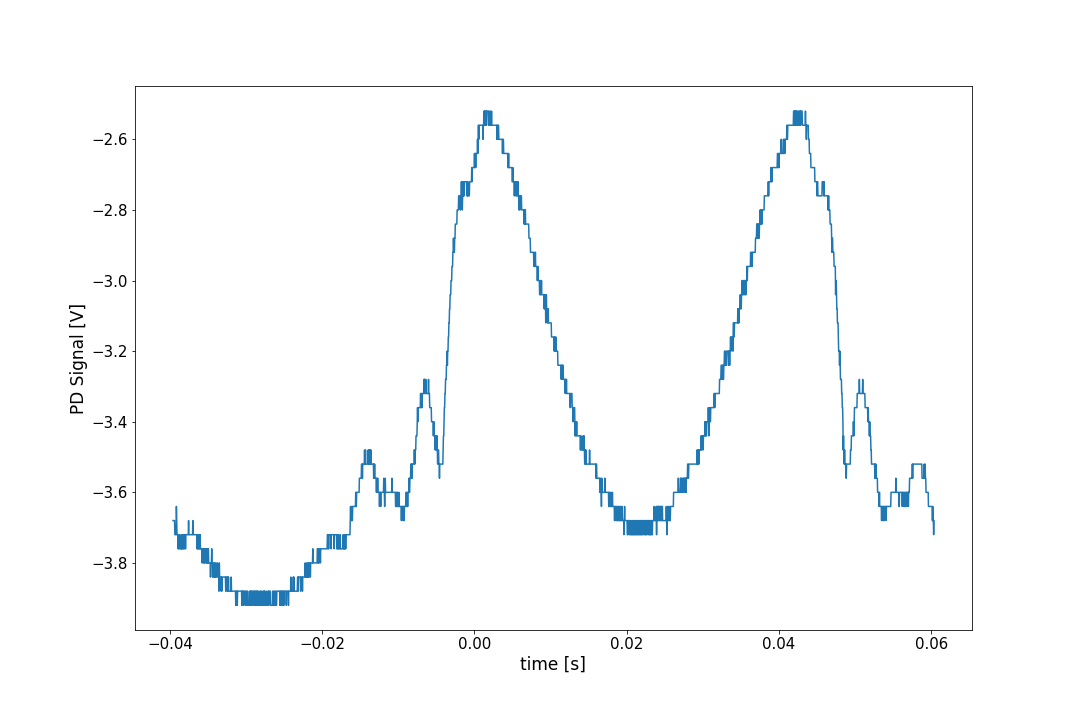
\includegraphics[keepaspectratio,  scale=0.35,  angle=0]
                          {figures/saturated-absorption/Repump_PD_signal.png}
                          \caption{PDで観測されたCs原子の超微細構造(リポンプレーザー)}
                          \label{Repump_PD_signal}
      \end{minipage}
    \end{tabular}
\end{figure}




\newpage
\chapter{光周波数コムのテーパーアンプによる増幅実験}
\section{光周波数コムのテーパーアンプによる増幅}
 二光子励起の励起効率の式(\ref{ResonanceRabi}), (\ref{ExcitationRate})から分かる通り、励起効率はコムの強度の二乗に比例する。そのため、二光子のレーザー冷却を行うに当たり、高効率の二光子励起を実現するためには高強度のレーザーを用意することが非常に重要である。そのため今回の実験では、光周波数コムから得られた光をTAを用いて増幅するという手段を用いる。しかし、通常TAはcwレーザーを増幅するために用いられるため、光周波数コムの増幅に用いた場合にどのような振る舞いを見せるかについての過去の研究は限られており、異なる繰り返し周波数に対してのTAの利得を調べた研究はまだない。今回の実験では繰り返し周波数の異なる光周波数コムに対してTAの増幅の様子を測定した。

\newpage
\section{テーパーアンプのマウンターの組み立て}
 今回の実験では、Cs原子のレーザー冷却に必要なパワーを得るためにTAを用いた。光周波数コムのから$760 \mathrm{nm}$付近の波長と$890 \mathrm{nm}$付近の波長を切り出し増幅した。$890 \mathrm{nm}$側の増幅に用いるTAのチップのマウンターに関しては、設計と組み立てを行った。TAのチップはeagleyard社のEYP-TPA-0915-01500-3006-CMT03-0000を用いた。TAのチップの構造は図\ref{TA_chip_ds}のようになっている。\\
\begin{figure}[htbp]
 \begin{center}
  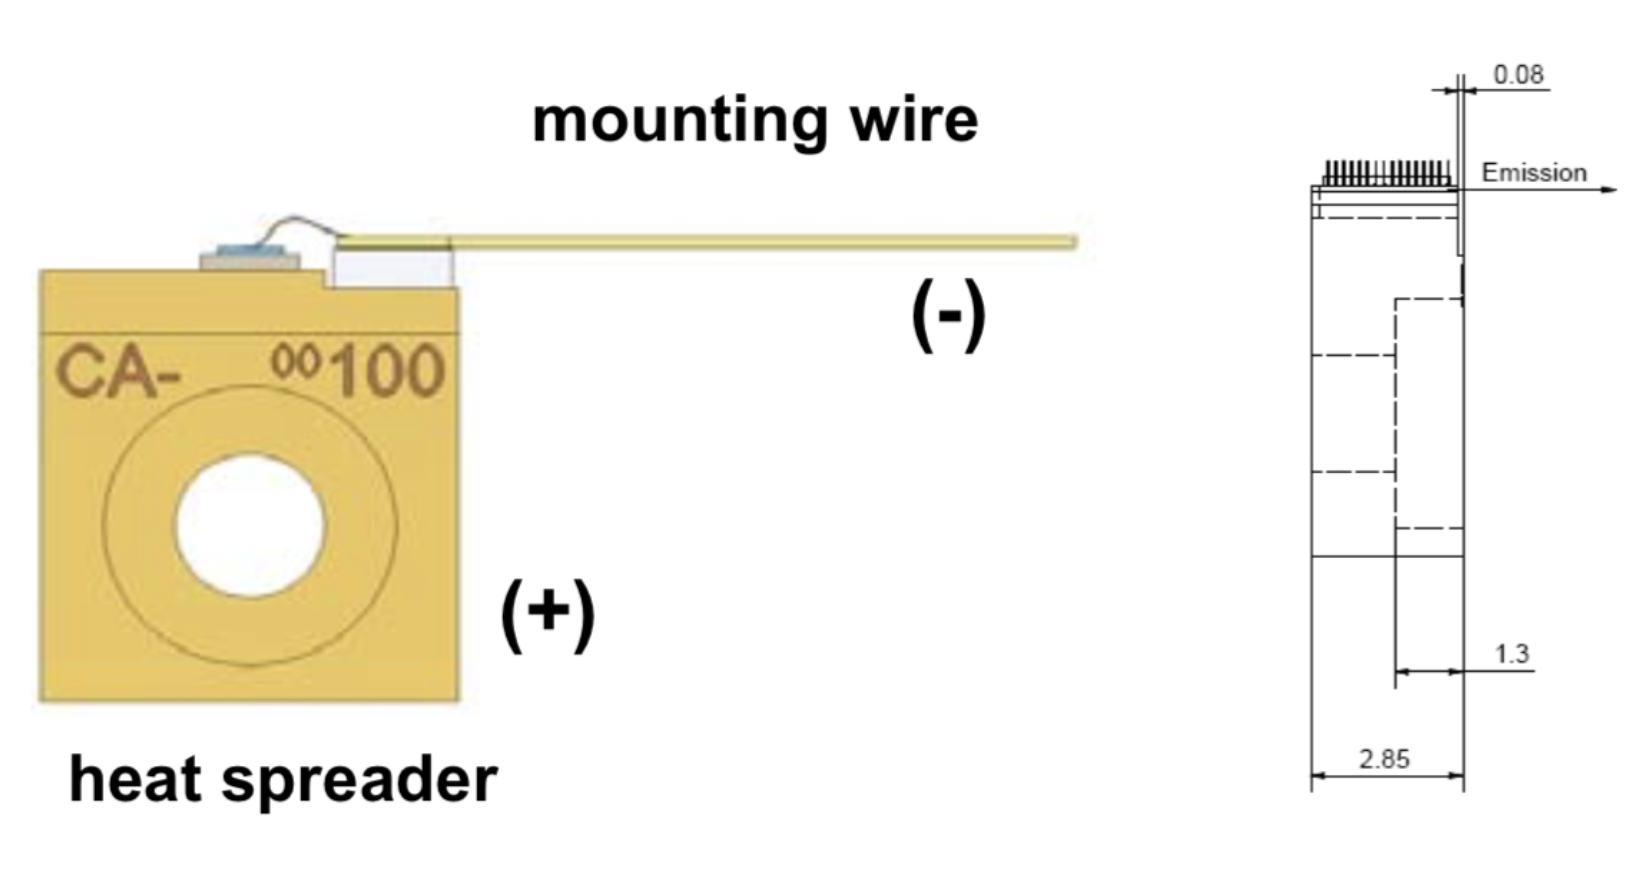
\includegraphics[width=70mm]{figures/chapter4/TA_chip_ds.png}
\end{center}
 \caption{TAチップの構造図(eagleyard社のデータシートから引用)}
 \label{TA_chip_ds}
\end{figure}
 TAチップのマウンターの構造は図\ref{TA_mounter_photo_comments},\ref{TA_mounter_structure}のようになっている。ただし、TAチップの入力光をマスター光、出力光をスレーブ光と呼ぶ。TAチップは銅のブロックにコリメーションレンズ2枚と共に取り付けられており、そこに温度センサーと直流電源からのSMAケーブルが繋がっている。この銅製のブロックをアルミニウム製のブロックを介して光学定盤に固定している。二つのブロックの間にペルチェ素子を挟み、温度を制御している。なお、レンズのマウンターにはアルミニウムを使用している。

\begin{figure}[htpb]
  \centering
    \begin{tabular}{c}

%----- TAチップマウンターの概観 -----

      \begin{minipage}{0.50\hsize}
        \centering
          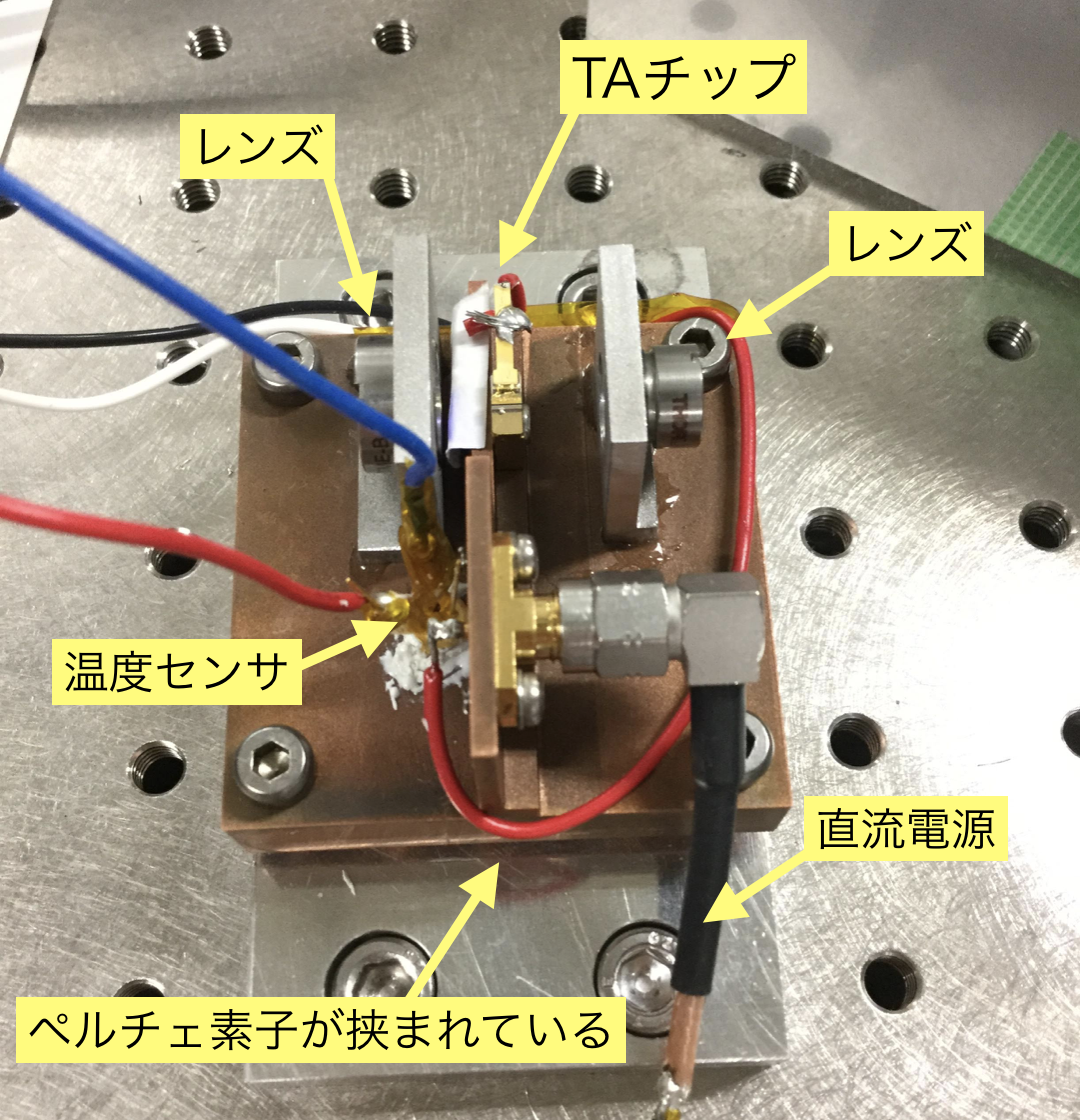
\includegraphics[keepaspectratio,  scale=0.30,  angle=0]
                          {figures/chapter4/TA_mounter_photo_comments.png}
                          \caption{TAチップマウンターの概観}
                          \label{TA_mounter_photo_comments}
      \end{minipage}

%----- TAチップマウンターの構造図 -----

      \begin{minipage}{0.50\hsize}
        \centering
          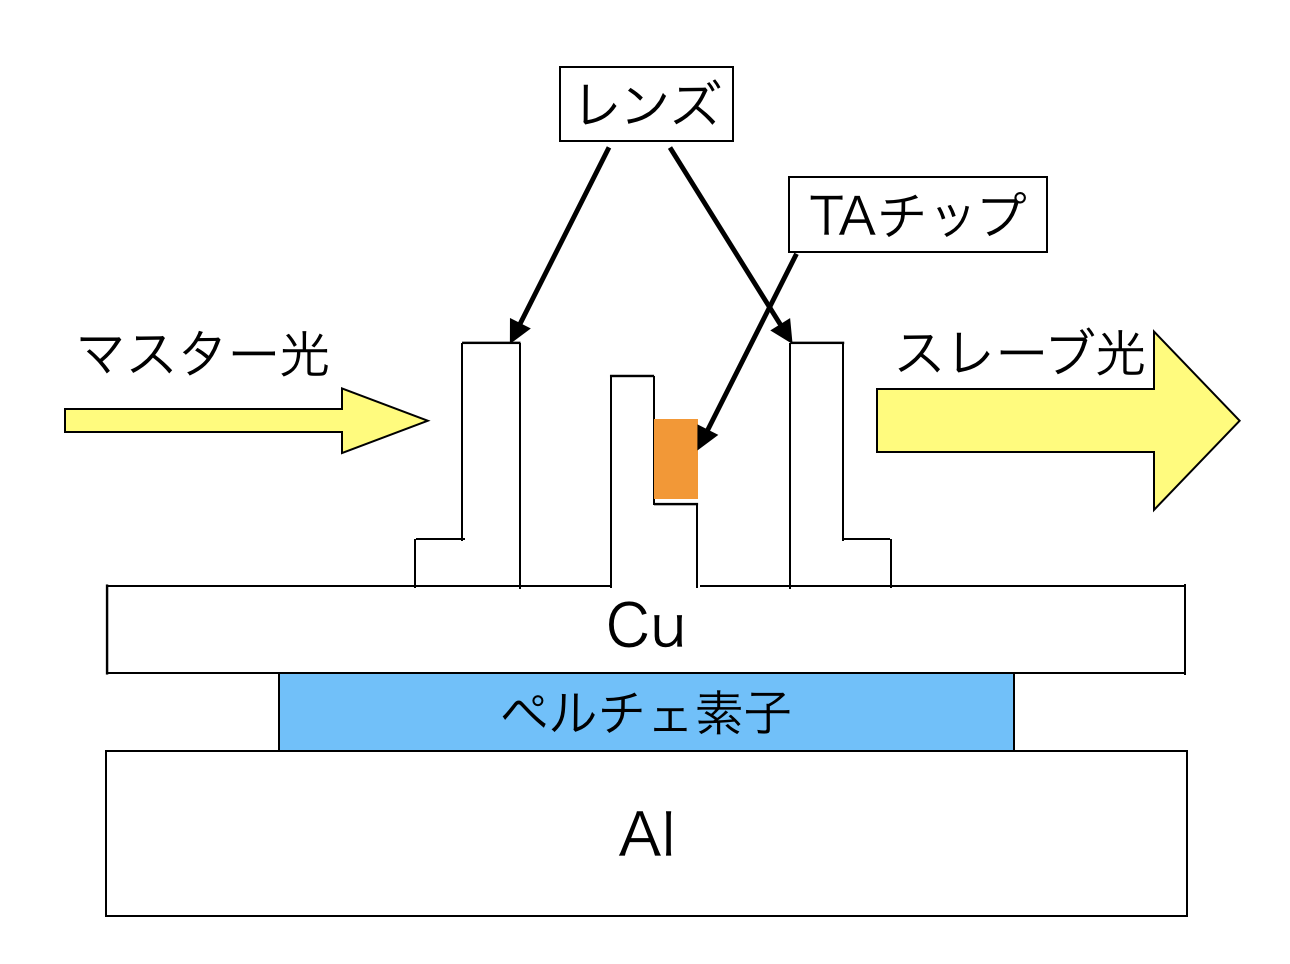
\includegraphics[keepaspectratio,  scale=0.35,  angle=0]
                          {figures/chapter4/TA_mounter_structure.png}
                          \caption{TAチップマウンターの構造図}
                          \label{TA_mounter_structure}
      \end{minipage}

    \end{tabular}
\end{figure}
\newpage
 なお、実際に使用する際には、図\ref{TA_case}のようにアクリルボードでケースを作り使用した。 また、スレーブ光の形状は光の回折の効果から楕円状になっているため、垂直方向のコリメーションを銅ブロック状のレンズで行い、水平方向のコリメーションを追加のシリンドリカルレンズで行う必要がある。\\
\begin{figure}[htbp]
 \begin{center}
  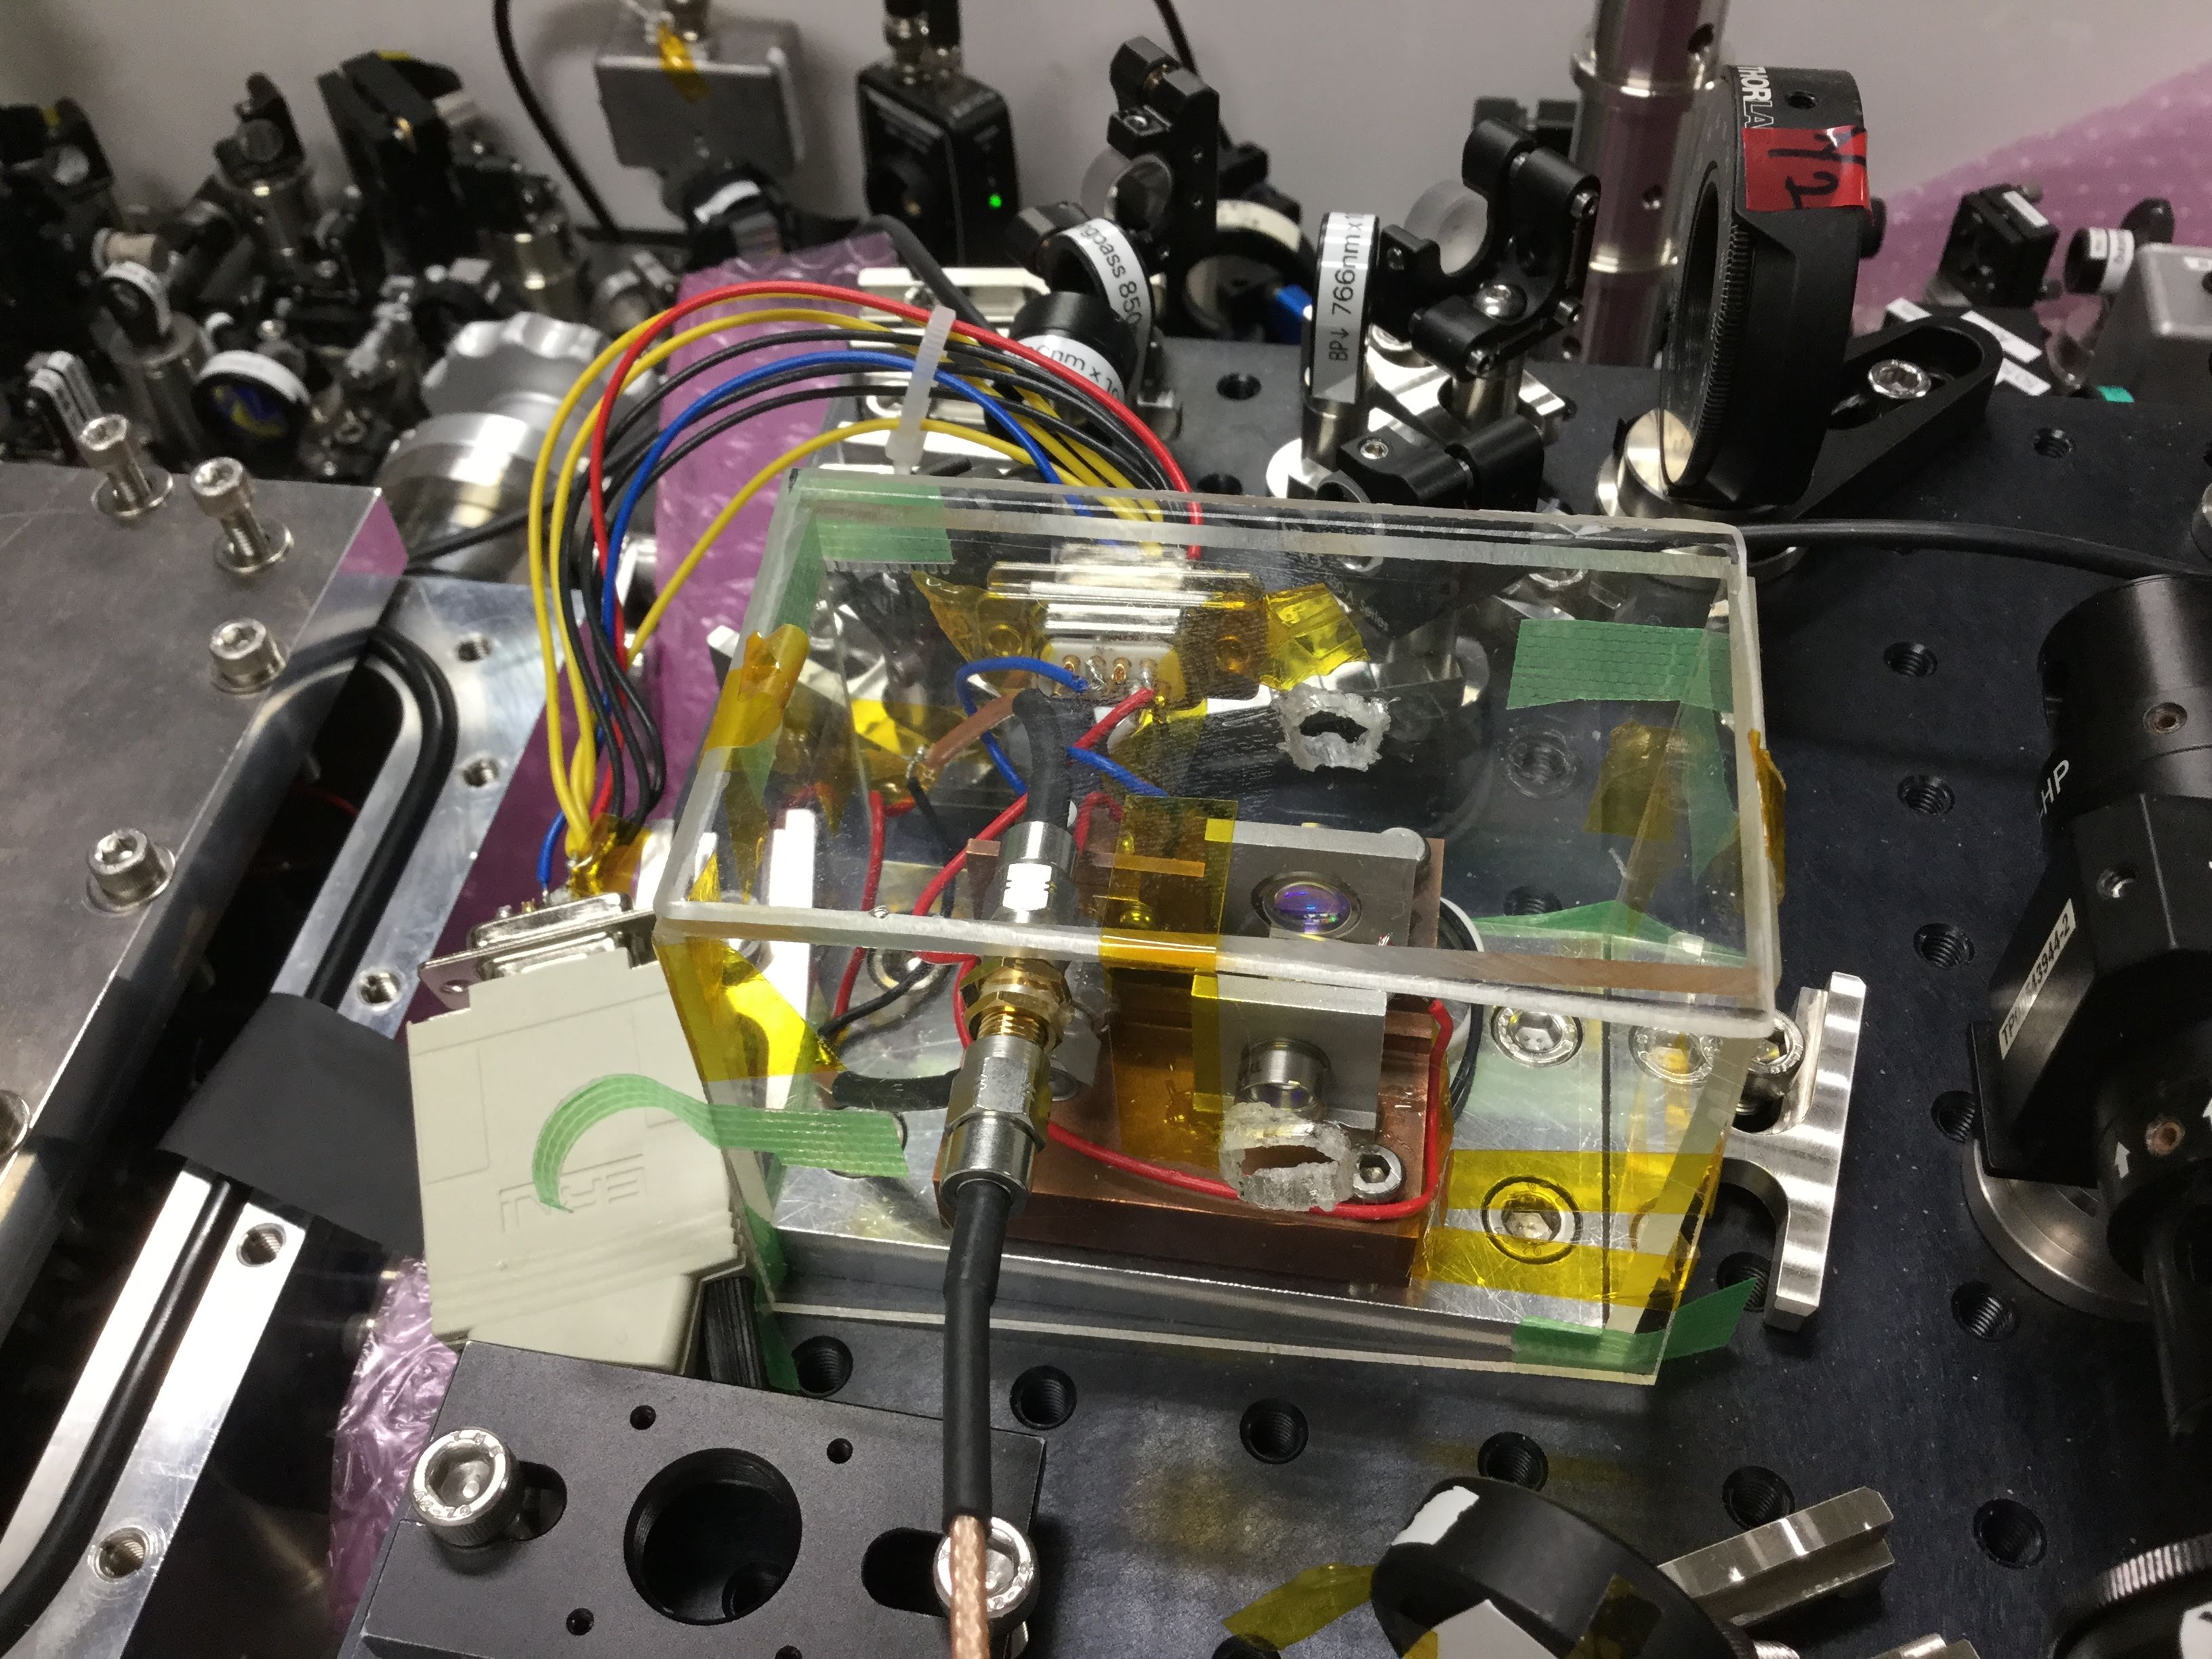
\includegraphics[width=75mm]{figures/chapter4/TA_case.jpg}
\end{center}
 \caption{実際に使用時のTAの様子}
 \label{TA_case}
\end{figure}



\newpage
\section{増幅実験の測定手法}
\subsection{繰り返し周波数の異なるコムでの増幅の比較}
 繰り返し周波数が$120$ MHzと$1.6$ GHzの二台のコムの、$766$ nmを中心波長とする幅$10$ nmのバンドパスフィルター(BPF)を通過した光をTAで増幅させ、マスター光とスレーブ光のパワーを測定した。その際に、BPF通過前のコムのスペクトルと、テーパーアンプの入り口と出口でのコムのスペクトルも測定を行った。その際の光学系は図\ref{760_amp_diagram}, \ref{760_astro_amp_diagram}に示している。繰り返し周波数$120$ MHzのコムを用いた実験ではアイソレータを入れないでTAの実験を行ったところ、TAからの戻り光がコムに光フィードバックをもたらしcw的発振を引き起こすことが観測された。このためアイソレータを使用している。一方で、くり返し周波数が$1.6$ GHzのコムの実験ではアイソレータを使用しなくても、TAからの戻り光がコムの共振器まで戻らずcw的な発振を起こさなかったため、アイソレータは使用しなかった。\\
\subsection{自作のTAでの890nm付近のコムの増幅}
 また、自作したTAで繰り返し周波数が$1.6$ GHzのコムの、$890$ nmを中心波長とする幅$10$ nmのBPFを通過した光を増幅させ、マスター光とスレーブ光のパワーの測定を行った。その際の光学系は図\ref{890_astro_amp_diagram}に示した。
\begin{figure}[htpb]
  \centering
    \begin{tabular}{c}
\begin{comment}
%----- 繰り返し周波数$120$ MHzのコムの$766$ nm付近の光を増幅した際の光学系 -----

      \begin{minipage}{0.5\hsize}
        \centering
          \includegraphics[keepaspectratio,  scale=0.16,  angle=0]
                          {figures/760_amp_experiment_comment.png}
                          \caption{繰り返し周波数$120$ MHzのコムの$766$ nm付近の光を増幅した際の光学系}
                          \label{760_amp_experiment_comment}
      \end{minipage}

%----- 上の写真の概略図 -----
\end{comment}

      \begin{minipage}{0.5\hsize}
        \centering
          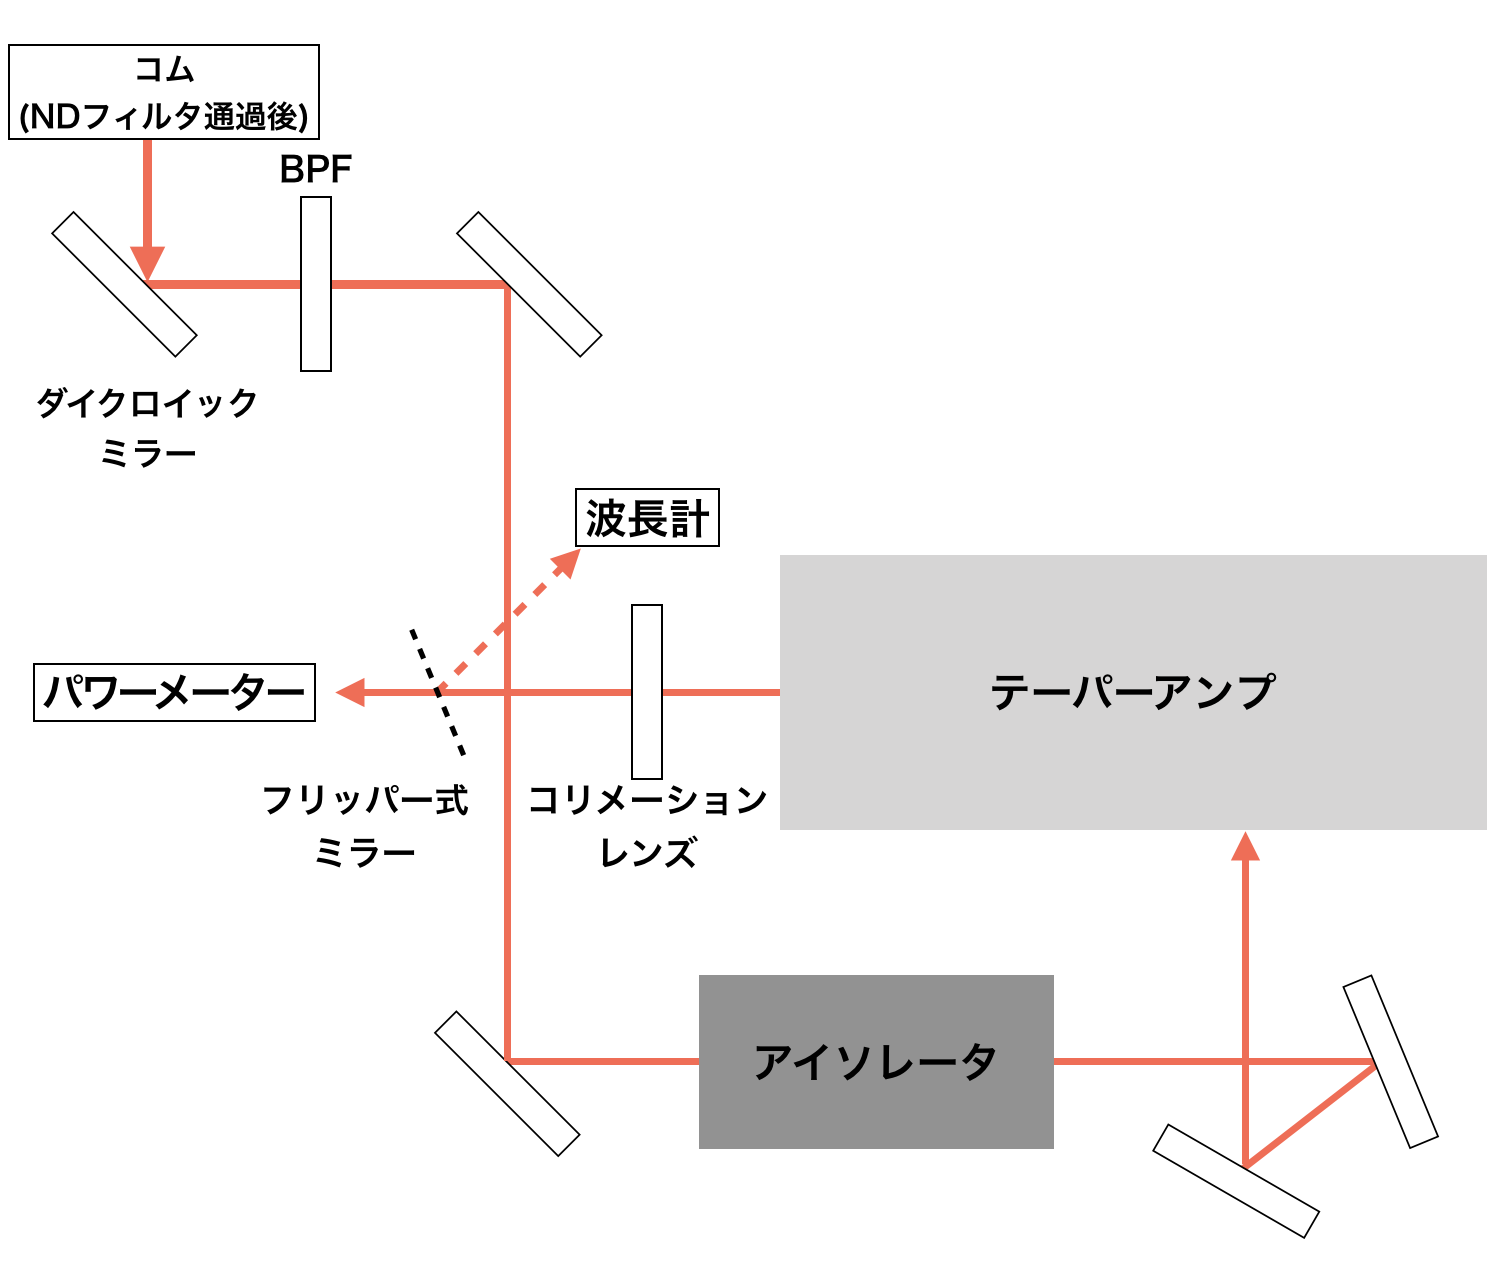
\includegraphics[keepaspectratio,  scale=0.25,  angle=0]
                          {figures/chapter4/760_amp_diagram.png}
                          \caption{繰り返し周波数$120$ MHzのコムの$766$ nm付近の光を増幅した際の光学系\\(アイソレータ有り)}
                          \label{760_amp_diagram}
      \end{minipage}

      \begin{minipage}{0.5\hsize}
        \centering
          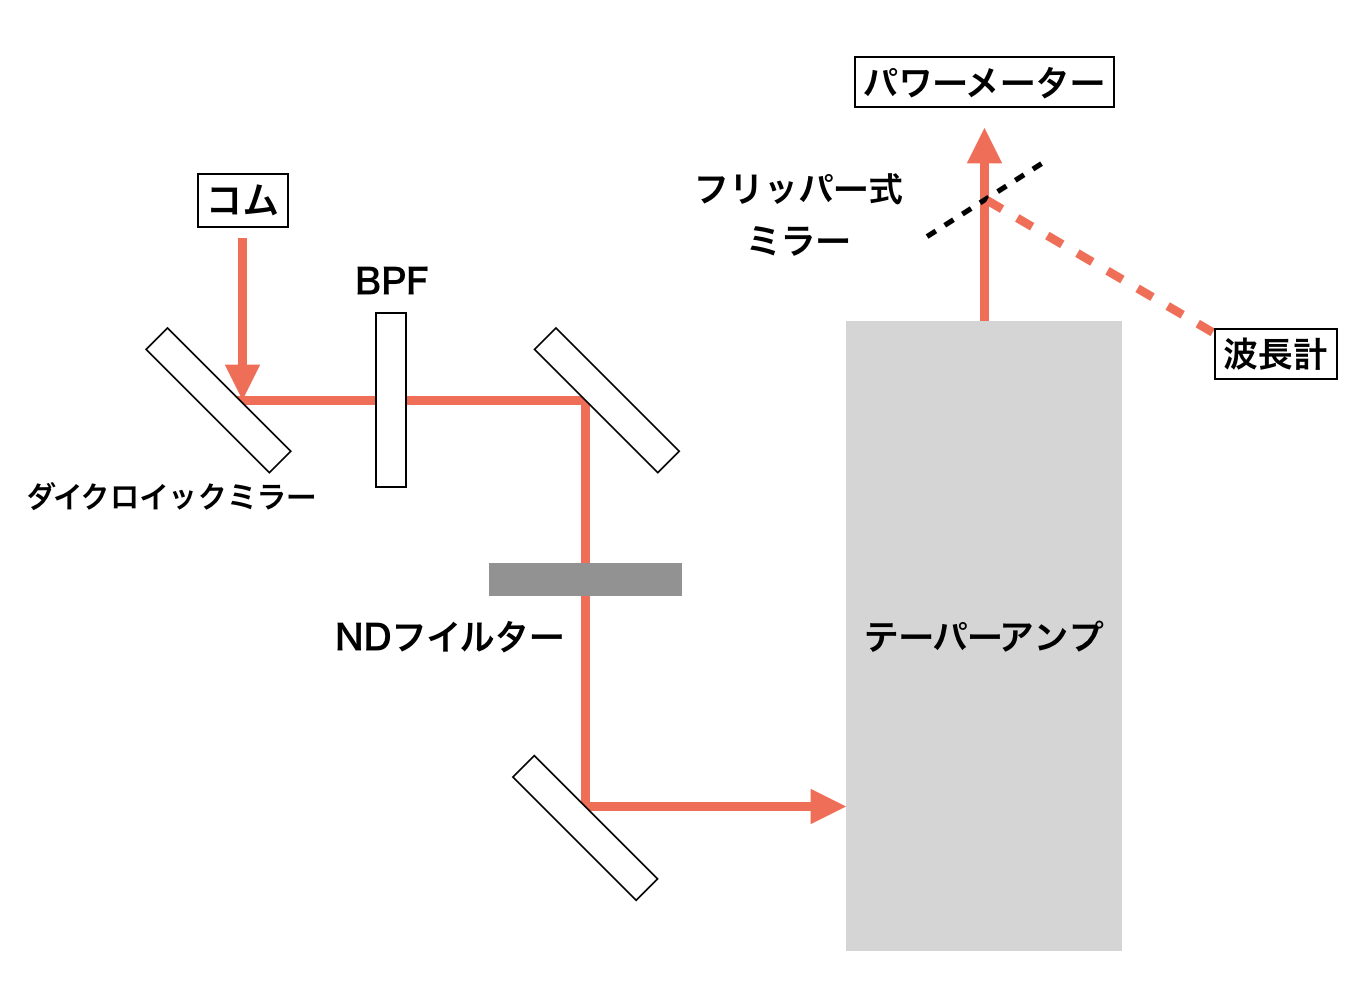
\includegraphics[keepaspectratio,  scale=0.33,  angle=0]
                          {figures/chapter4/760_astro_amp_diagram.png}
                          \caption{繰り返し周波数$1.6$ GHzのコムの$766$ nm付近の光を増幅した際の光学系}
                          \label{760_astro_amp_diagram}
      \end{minipage}\\
      \\

      \begin{minipage}{0.5\hsize}
        \centering
          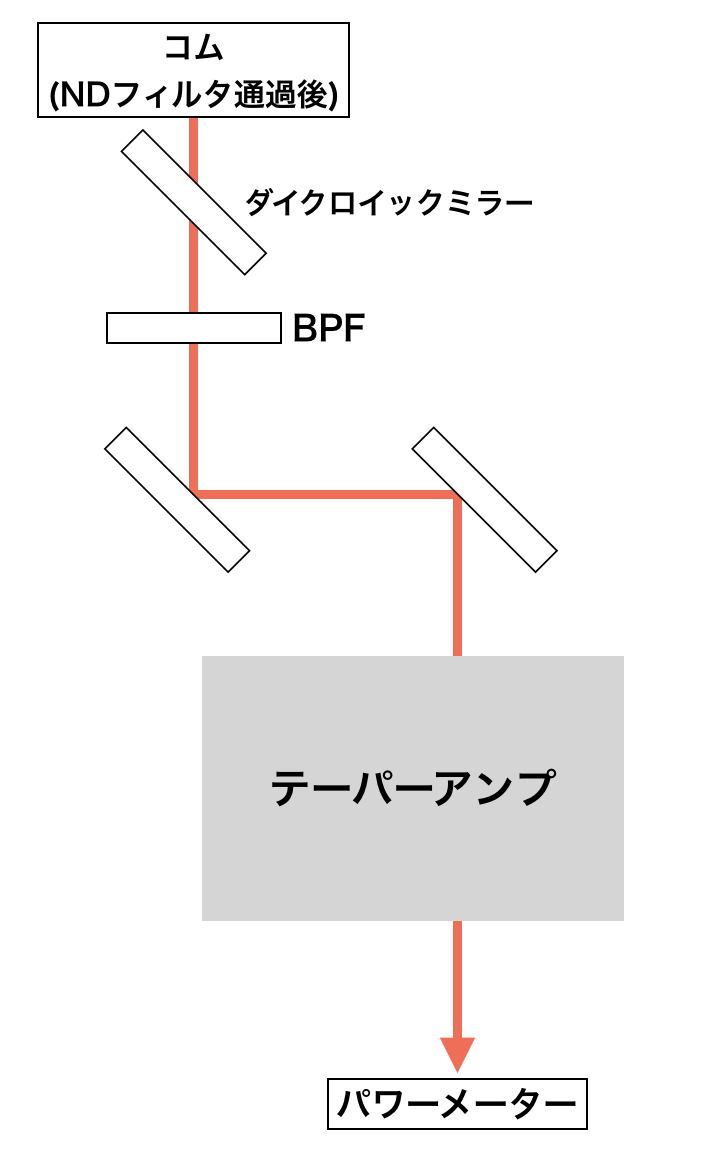
\includegraphics[keepaspectratio,  scale=0.3,  angle=0]
                          {figures/chapter4/890_astro_amp_diagram.png}
                          \caption{繰り返し周波数$1.6$ GHzのコムの$890$ nm付近の光を増幅した際の光学系}
                          \label{890_astro_amp_diagram}
      \end{minipage}

    \end{tabular}
\end{figure}
\newpage
\subsection{ダブルパスによる増幅}
  TAは通常ゲイン領域が細い方からマスター光を入射し、ゲイン領域の広い方からスレーブ光を出力するという使用法をする。しかし、通常の出力側からマスター光を入射し通常の入力側から出た光をミラーで打ち返し再度通常の入力側に光を入射させ、二度ゲイン領域を通過させ増幅するという手法がある。この光学系の配置をダブルパスといい、これに対して通常の配置をシングルパスと呼ぶことがある。ダブルパスでのcwレーザーのTAの増幅の振る舞いについては過去の研究\cite{doi:10.1063/1.3501966}があり、通常cw光でTAを飽和させるには数十ワットのマスター光が必要となるが、ダブルパスの場合だと$200 \mathrm{\mu W}$のマスター光で飽和させることが出来ることが分かっている。また、スペクトルの面でもキャリアの周波数的に幅の広い自然放出が抑えられることが分かっている。このように、ダブルパスによるメリットは多いが光周波数コムの増幅にダブルパスを用いている研究はまだない。そのため今回の実験では,繰り返し周波数$1.6$ GHzの$761$ nmから$771$ nmのコムをダブルパスにより増幅する実験を行った。

 \begin{figure}[htbp]
  \begin{center}
   \includegraphics[width=120mm]{figures/chapter4/doublepass_photo.png}
 \end{center}
  \caption{ダブルパス配置の光学系}
  \label{doublepass_photo}
 \end{figure}

\newpage
\section{測定結果}
\subsection{アイソレータなしの場合のコムのスペクトルの変化}
 図\ref{spectrum_current_MODORI}はマスター光入射時にアイソレータを使用しなかった時の、光周波数コムのキャビティの出力口におけるスペクトラムをTAに印加する電流の大きさを変えつつ分光器で測定したものである。TAの印加電流をあげていくと$770$ nm付近でcw的な発振を起こしていることが分かる。これはTAの入射口から出た自然放出の光が光周波数コムの共振器まで戻り、光フィードバックを起こしているものと考えられる。\\
 そのためマスター光入射時にアイソレータを通過させたところ、スペクトルは図のようになった。このようなcw的な発振は観測されなかった。
\begin{figure}[htbp]
 \begin{center}
  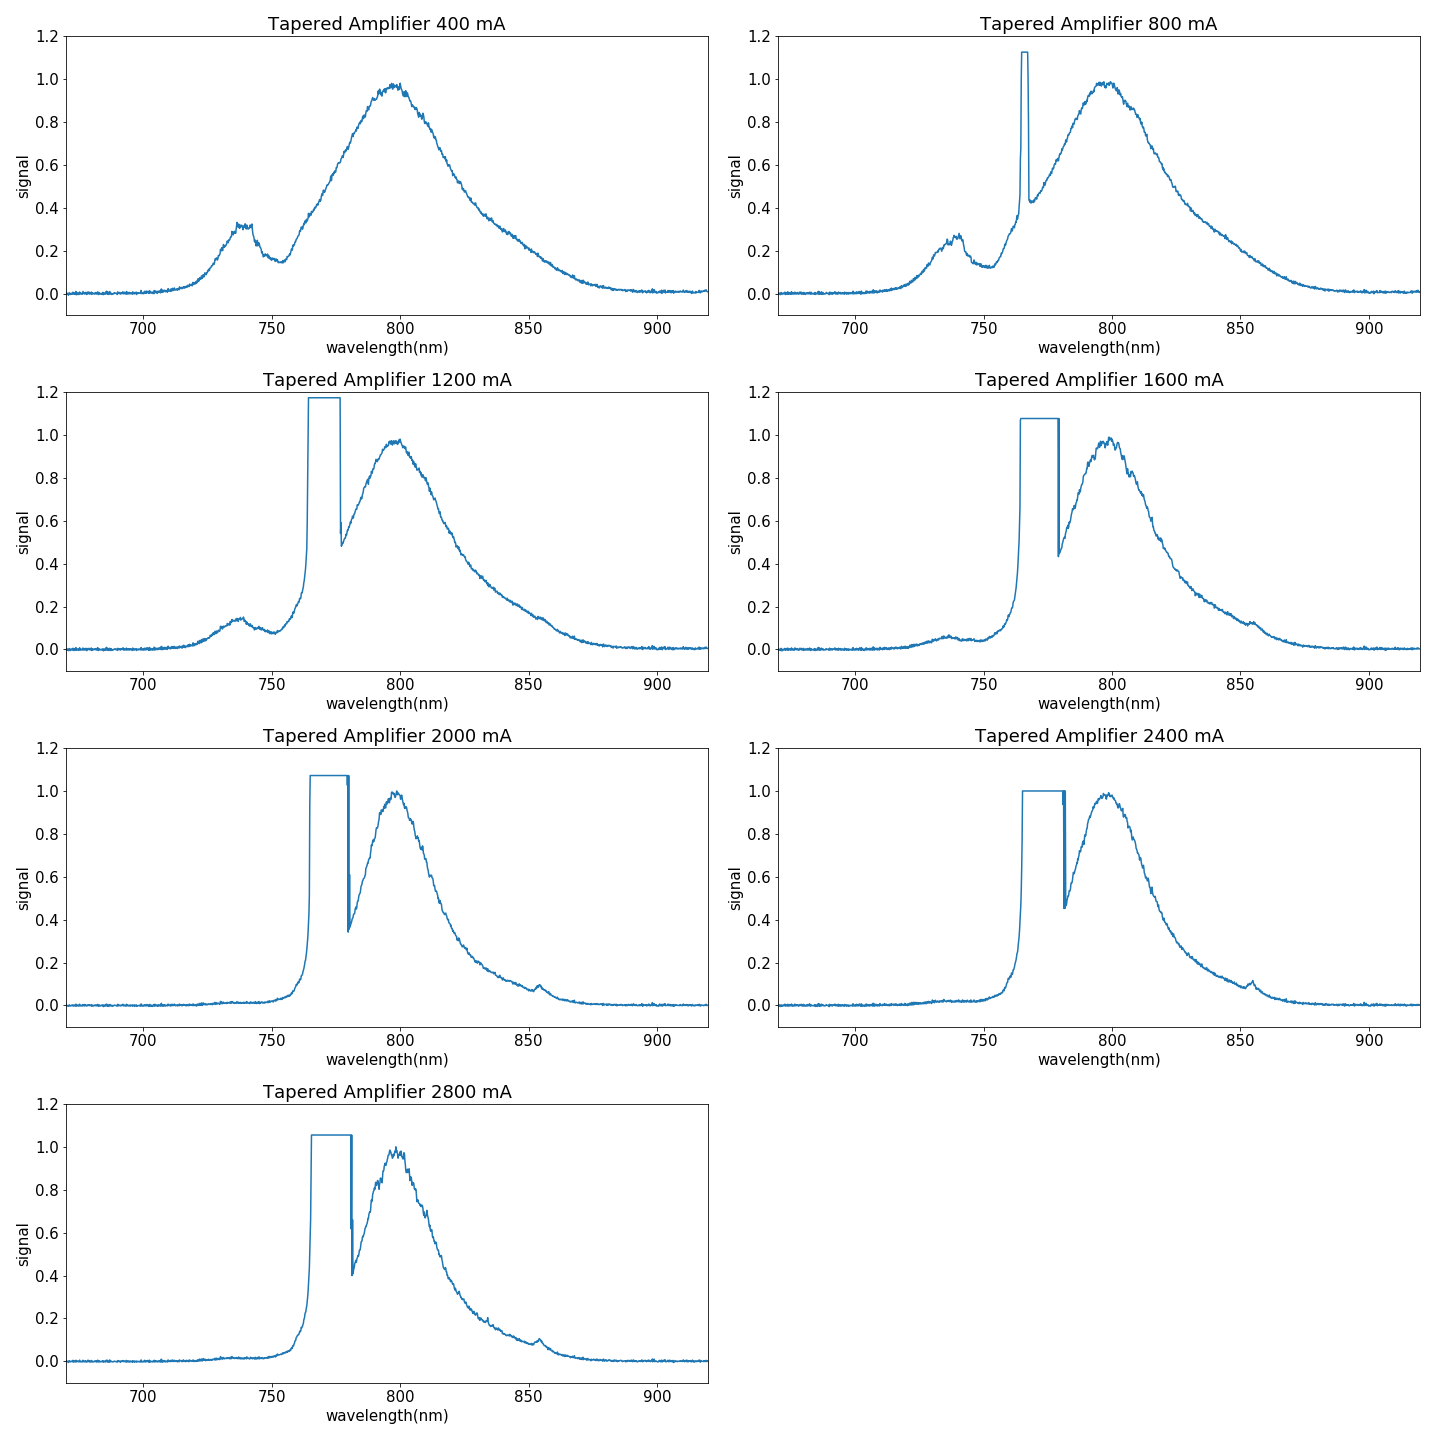
\includegraphics[width=140mm]{figures/chapter4/spectrum_current_MODORI.png}
\end{center}
 \caption{戻り光の影響によるコムのスペクトルの変化}
 \label{spectrum_current_MODORI}
\end{figure}
\newpage
\subsection{繰り返し周波数の異なるコムの増幅}

図\ref{pulse_power-gain-comparison}は766nm側のコムを増幅した際の利得のパルスエネルギー依存性依存性を二つの繰り返し周波数に応じて比較したものである。繰り返し周波数$120 \mathrm{MHz}$の利得をみると、パルスエネルギーの増加に対して利得が低下していく様子がわかる。これは、各パルスに含まれる光子数に対して励起状態にあるキャリア数が足りておらずパルスエネルギーの増加に対して利得を保てていないと考えられる。それに対し、繰り返し周波数$1.6 \mathrm{GHz}$のコムの利得は$120$ MHzのコムの利得を下回っている。これはパルスの時間間隔が$630$ ps程度で短く、十分な反転分布が励起されていないことが原因ではないかと考えられる。\\
 また、スレーブ光強度のマスター光強度依存性を二台のコムで比較すると図\ref{M-S_power-comparison}のようになる。同じマスター光強度で比較すると、繰り返し周波数が$1.6$ GHzのコムのスレーブ光強度が上回っていることがわかる。これは同じ光強度の場合、繰り返し周波数が$120$ MHzのコムでは繰り返し周波数が$1.6$ GHzのコムに比べ一つのパルスに含まれる光子数が多いが、TA内のキャリア数が少ないので誘導放出に使われない光子数が多くなってしまい光が増幅されないことが原因だと考えられる。一方、$1.6$ GHzのコムでは一パルスあたりの光子数が少ないため、無駄になる光子が少なく効率よく増幅することができると考えられる。

\begin{figure}[htpb]
  \centering
    \begin{tabular}{c}

%----- 写真 -----

      \begin{minipage}{0.50\hsize}
        \centering
          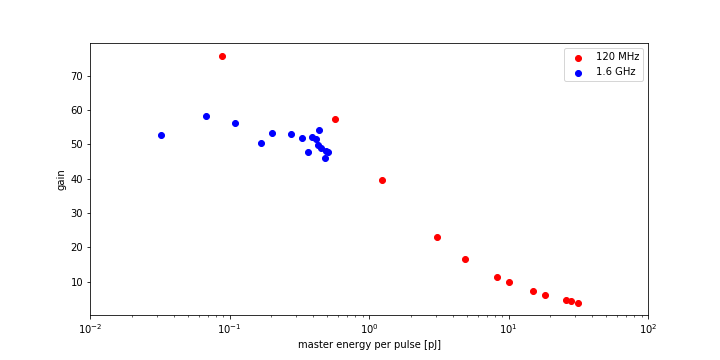
\includegraphics[keepaspectratio,  scale=0.30,  angle=0]
                          {figures/chapter4/pulse_power-gain-comparison.png}
                          \caption{二台のコムにおけるTAの利得のパルスエネルギー依存性の比較}
                          \label{pulse_power-gain-comparison}
      \end{minipage}

%----- PD Signal -----

      \begin{minipage}{0.50\hsize}
        \centering
          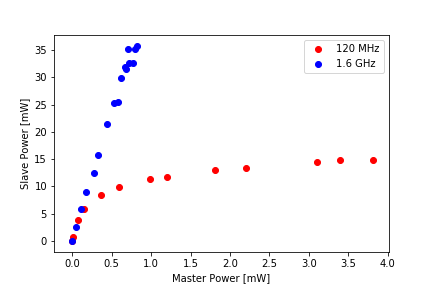
\includegraphics[keepaspectratio,  scale=0.35,  angle=0]
                          {figures/chapter4/M-S_power_comparison.png}
                          \caption{二台のコムにおけるスレーブ光強度のマスター光強度依存性の比較}
                          \label{M-S_power-comparison}
      \end{minipage} \\

      \begin{minipage}{0.50\hsize}
        \centering
          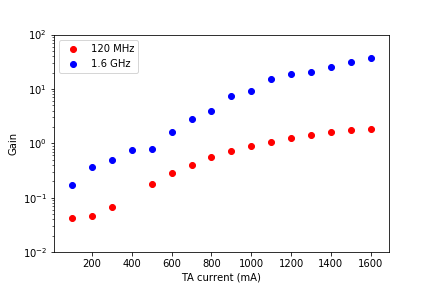
\includegraphics[keepaspectratio,  scale=0.35,  angle=0]
                          {figures/chapter4/TA_cuurent-gain_comparison.png}
                          \caption{二台のコムにおけるTAの利得の印加電流依存性の比較}
                          \label{TA_cuurent-gain_comparison}
      \end{minipage}
    \end{tabular}
\end{figure}
\subsection{繰り返し周波数$1.6$ GHzの$890$ nm付近のコムの増幅}
 繰り返し周波数$1.6$ GHzのコムの$885 \mathrm{nm}から 895 \mathrm{nm}$BPFを通過させた光をTAで増幅した結果を、図\ref{TA_power-current_3A_astro}, \ref{890TPA_power_dependence_0117}に示す。

\begin{figure}[htpb]
  \centering
    \begin{tabular}{c}

%----- 写真 -----

      \begin{minipage}{0.50\hsize}
        \centering
          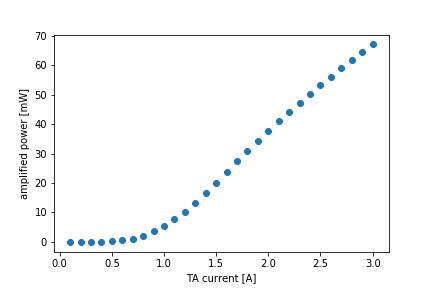
\includegraphics[keepaspectratio,  scale=0.50,  angle=0]
                          {figures/chapter4/TA_power-current_3A_astro.png}
                          \caption{890nm側の繰り返し周波数$1.6$ GHzでのTAのスレーブ光強度の電流依存性}
                          \label{TA_power-current_3A_astro}
      \end{minipage}

%----- PD Signal -----

      \begin{minipage}{0.50\hsize}
        \centering
          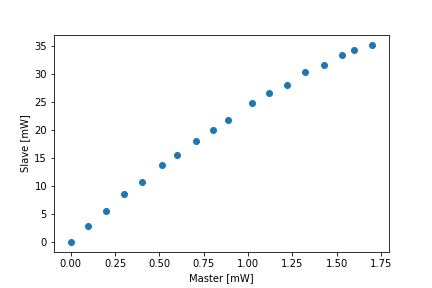
\includegraphics[keepaspectratio,  scale=0.5,  angle=0]
                          {figures/chapter4/890TPA_power_dependence_0117.png}
                          \caption{890nm側の繰り返し周波数$1.6$ GHzでのTAのスレーブ光強度のマスター光強度依存性}
                          \label{890TPA_power_dependence_0117}
      \end{minipage} \\

    \end{tabular}
\end{figure}

\subsection{ダブルパスでの増幅}


\newpage
\begin{figure}[htpb]
  \centering
    \begin{tabular}{c}

      \begin{minipage}{0.70\hsize}
        \centering
          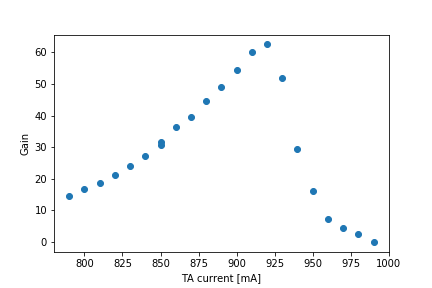
\includegraphics[keepaspectratio,  scale=0.5,  angle=0]
                          {figures/chapter4/double-pass_I-Gain.png}
                          \caption{ダブルパスでの利得の印加電流依存性}
                          \label{double-pass_I-Gain}
      \end{minipage}\\

      \begin{minipage}{1\hsize}
        \centering
          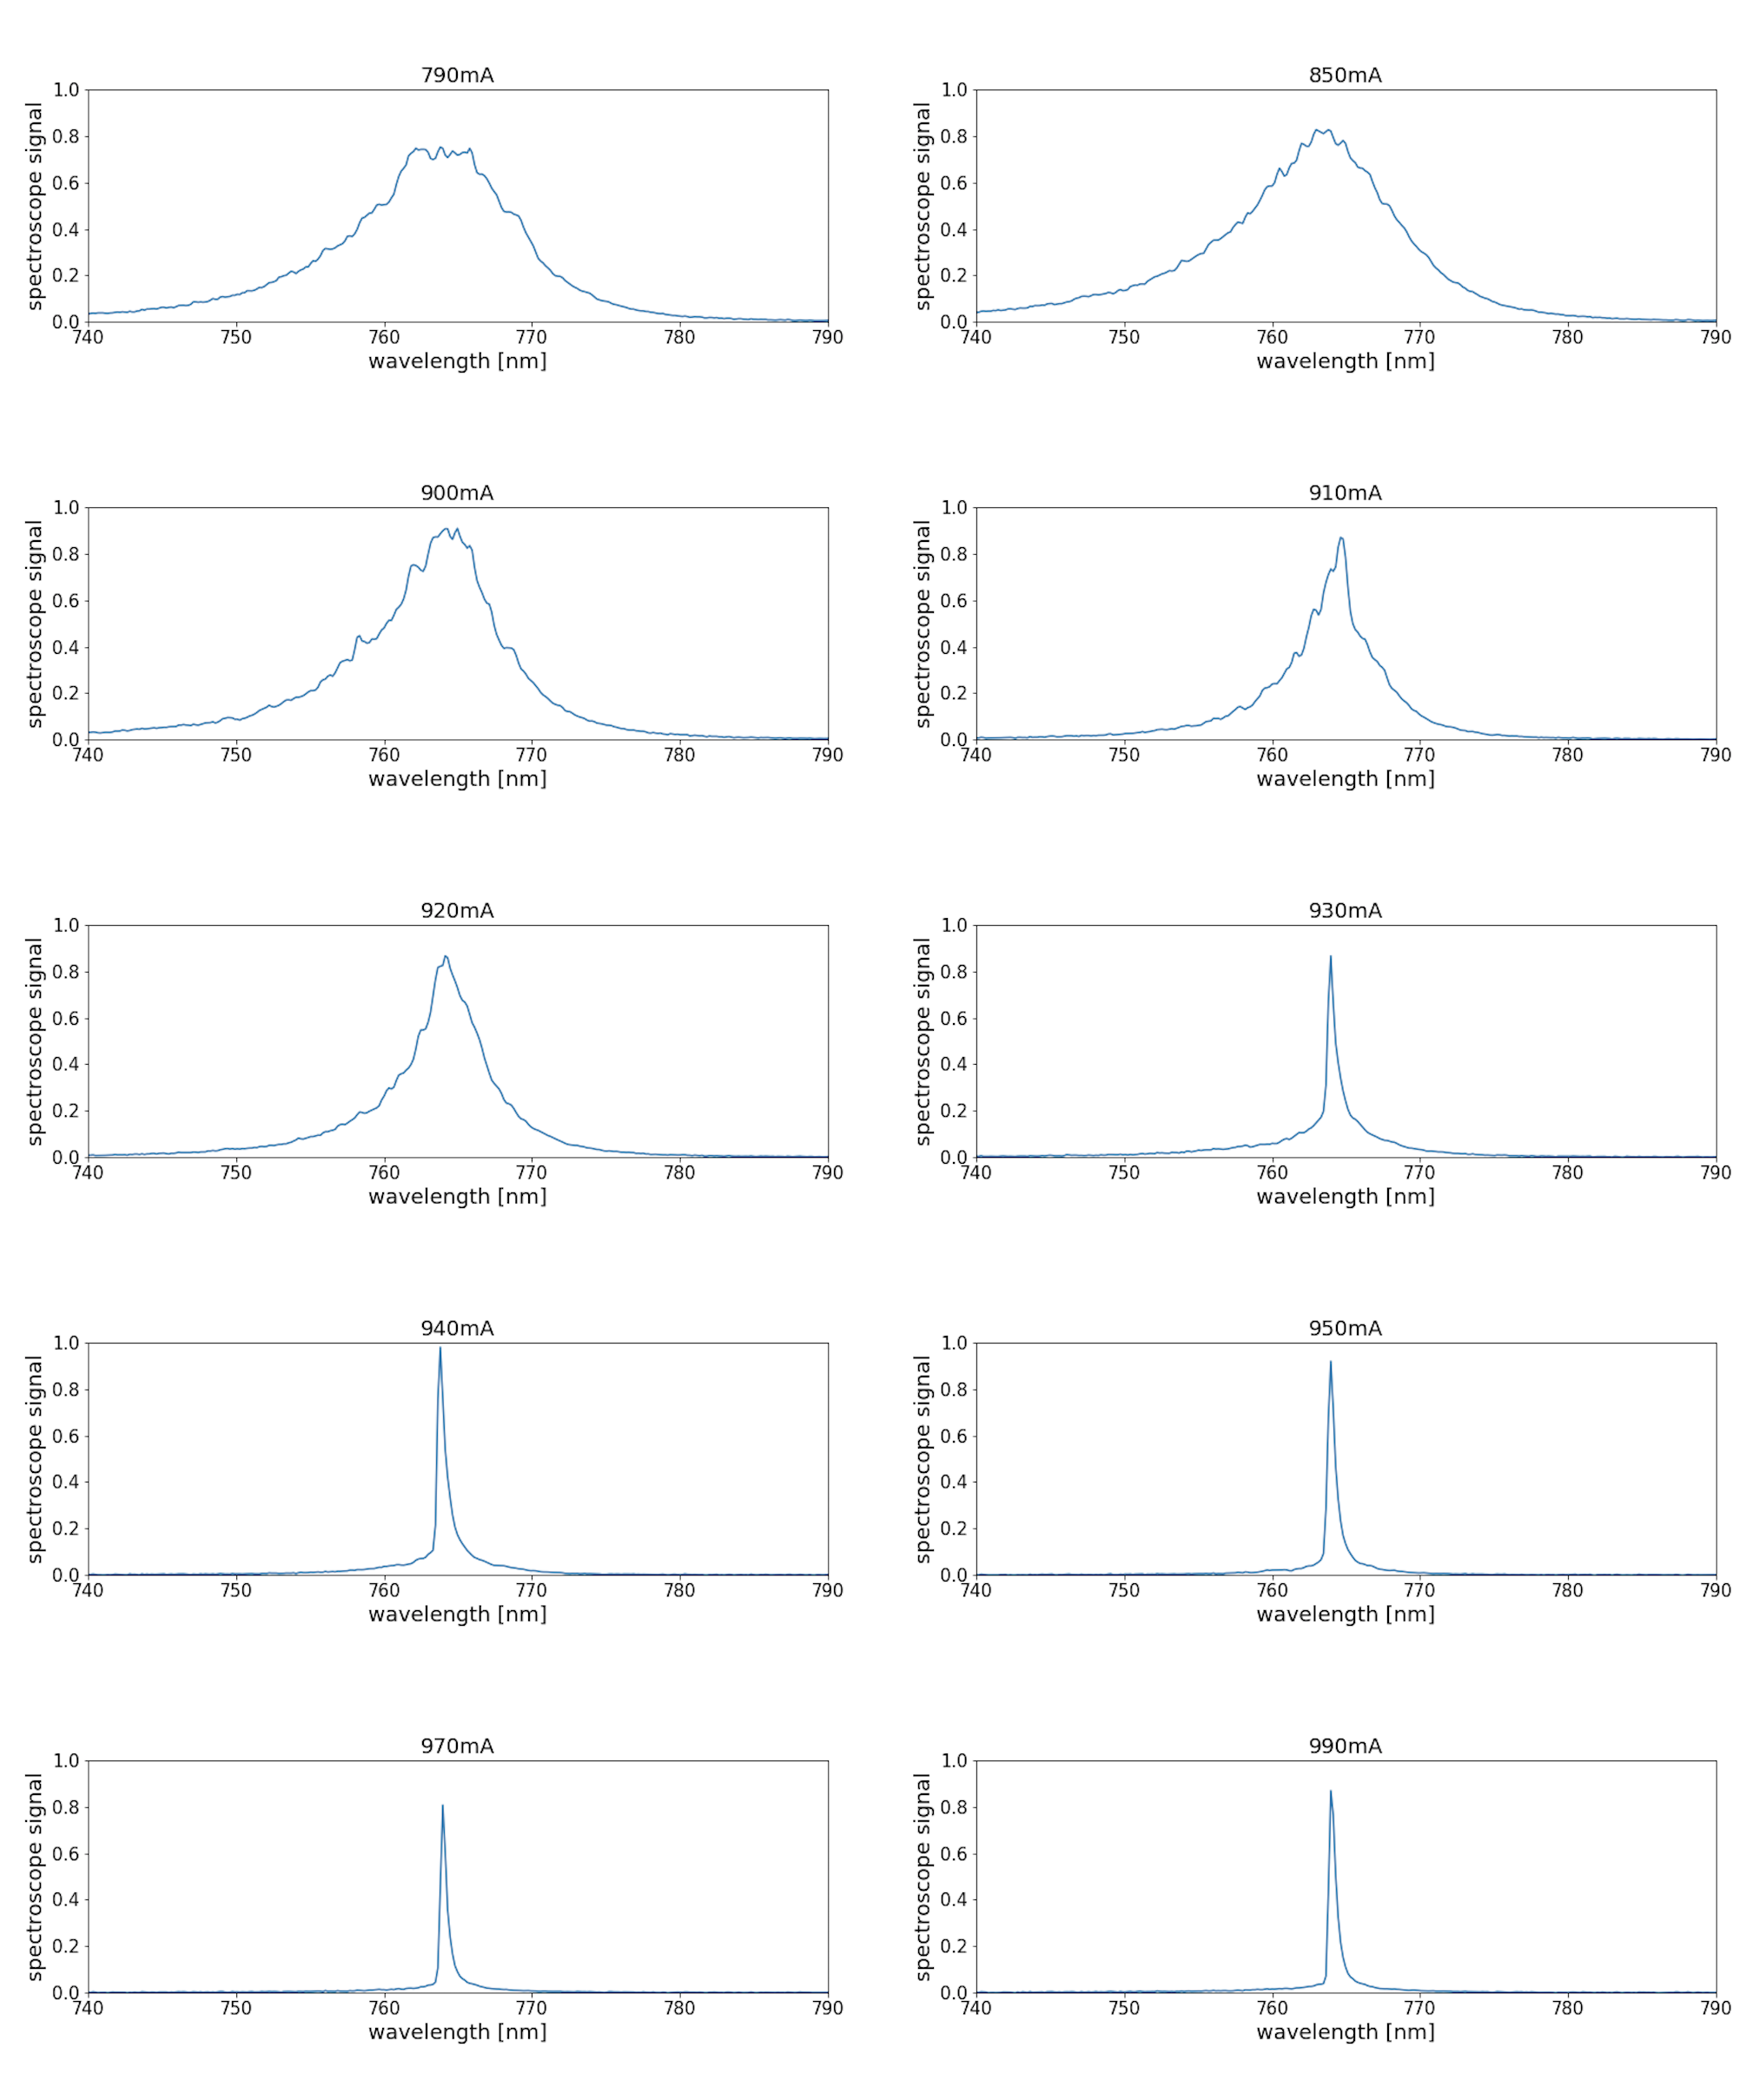
\includegraphics[keepaspectratio,  scale=0.340,  angle=0]
                          {figures/chapter4/double-pass-Slave-Spectrum.png}
                          \caption{ダブルパスでの各印加電流におけるスレーブ光のスペクトル}
                          \label{double-pass_I-Slave}

      \end{minipage}


    \end{tabular}
\end{figure}



\chapter{まとめと展望}






\bibliography{reference}
\end{document}
